\chapter{TELAAH PUSTAKA}
\label{cha:2-TelaahPustaka}

\vspace{1cm}
\section{\textit{Computer Vision}}
\hspace{1,2cm}\textit{Computer Vision} atau visi komputer adalah bidang kecerdasan buatan (AI) yang memungkinkan komputer dan sistem memperoleh informasi bermakna dari gambar digital, video, dan input visual lainnya, dan mengambil tindakan atau membuat rekomendasi berdasarkan informasi tersebut. Jika kecerdasan buatan memungkinkan komputer untuk berpikir, visi komputer memungkinkan untuk melihat, mengamati, dan memahami (IBM, 2020).

\textit{Computer vision} bekerja hamper sama dengan visi manusia, kecuali manusia memiliki permulaan. Penglihatan manusia memiliki keunggulan konteks seumur hidup untuk melatih cara membedakan objek, seberapa jauh jaraknya, apakah bergerak, dan apakah ada yang salah dalam sebuah gambar. \textit{Computer vision} melatih mesin untuk melakukan fungsi-fungsi melatih mesin untuk melakukan fungsi-fungsi ini, tetapi ia harus melakukannya dalam waktu yang jauh lebih singkat dengan kamera, data, dan algoritma daripada retina, saraf, optic, dan korteks visual karena sistem yang dilatih untuk memeriksa produk atau mengamati asset produksi dapat menganalisis ribuan produk atau proses dalam satu menit, memperhatikan cacat atau masalah yang tidak terlihat, sistem tersebut dapat dengan cepat melampaui kemampuan manusia. 

Memahami dan menentukan tugas visi komputer tertentu dapat memfokuskan dan memvalidasi proyek dan aplikasi, serta mempermudah untuk memulai. Hal dasar untuk \textit{computer vision} adalah \textit{object detection}, beberapa tugas visi komputer lainnya, seperti \textit{image classification, object detection, object tracking}, dan \textit{content-based image retrieval} (U. Arshad, 2021).

\vspace{1cm}
\section{Pengertian Citra}
Citra didefinisikan sebagai fungsi dari dua variabel misalnya \textit{a(x,y)} dimana a sendiri sebagai amplitudo (misalnya kecerahan) citra pada koordinat (x,y) (I. T. Young et al, 1995). Citra digital a[m,n] merupakan citra dalam ruang diskrit 2D yang berasal dari citra analog a(x,y) di ruang kontinyu 2D melalui proses sampling yaitu yang biasa disebut sebagai digitalisasi. Sedangkan, menurut Maria citra digital adalah citra f(x,y) yang telah didiskritkan oleh pada koordinat spasial dan kecerahan. Citra digital direpresentasikan oleh \textit{array} dua dimensi atau sekumpulan \textit{array} dua dimensi dimana setiap \textit{array} merepresentasikan satu kanal warna. Nilai kecerahan yang didigitalkan dinamakan nilai tingkat keabuan (A. McAndrew, 2004).

Setiap elemen \textit{array} tersebut dinamakan piksel yang diambil dari istilah \textit{picture element}. Dimensi citra biasanya ditulis dengan format panjang x tinggi (misalnya 640 x 480 piksel). Namun, perlu diperhatikan dengan seksama bahwa secara matematis, definisi citra terlihat seperti di bawah ini, dimana x menunjukkan baris dan y menunjukkan kolom:

\[
f(x,y)=
\begin{bmatrix}
	f\left(0,0\right)  & f\left(0,1\right) & ... & f\left(0,N-1\right) \\ 
	f\left(1,0\right)  & f\left(1,1\right) & ... & f\left(1,N-1\right) \\
	... & ... & ... & .. \\
	f\left(M-1,0\right) & f\left(M-1,1\right) & ... & \ f\left(M-1,N-1\right)
\end{bmatrix}
\]

Seperti pada layar monitor, koordinat citra dimulai dari pojok kiri atas. Secara matematis dimulai dari (0,0) dan berakhir di (M-1, N-1), dimana M menunjukkan tinggi, dan N menunjukkan panjang.

\section{Pengolahan Citra}
\hspace{1,2cm}Pengolahan citra adalah pemrosesan citra, khususnya menggunakan komputer menjadi citra yang kualitasnya lebih baik. Pengolahan citr adikembangkan bertujuan untuk (M. Petrou, 1999):
\begin{enumerate}
	\item Untuk memperbaiki tampilan citra (\textit{image enhancement}).
	\item Untuk mengurangi ukuran file citra dengan tetap mempertahankan kualitas citra (\textit{image compression}).
	\item Untuk memulihkan citra ke kondisi semula (\textit{image restoration}). 
	\item Untuk menyoroti ciri tertentu dari citra agar lebih mudah untuk di analisis. 
\end{enumerate}

Pengolahan citra adalah cabang ilmu informatika untuk memperbaiki kualitas citra agar kualitasnya lebih baik atau lebih mudah diinterpretasi oleh manusia maupun komputer. Input dari program pengolahan citra adalah citra dan outputnya pun citra pula.

Pengolahan citra digital digunakan dalam berbagai bidang untuk mempermudah manusia dalam melakukan analisis dan pekerjaan. Bentuk aplikasi pengolahan citra digital yang digunakan bidang militer, industry, medis, transportasi, hukum dan keamanan, pemetaan, robotika, fotografi, film, pencarian gambar berdasarkan kandungan citra, dan pemahaman kandungan citra. Salah satu pemanfaatan teknologi pengolahan citra digital yaitu bisa memahami maksud dari sebuah citra. Apabila aplikasi diberikan input berupa gambar yang mampu mendefinisikan bahwa dalam gambar tersebut terdapat gambar yang mendapati objek, seperti kendaraan, jalan, buah, dan lainnya.

\section{\textit{Artificial Intelligence} (AI)}
\hspace{1,2cm}\textit{Artificial inlelligence} atau kecerdasan buatan adalah studi tentang teori dan pengembangan sistem komputer agar mampu melakukan tugas-tugas yang dahulu hanya dapat dilakukan oleh manusia. Seperti membadakan berbagai gambar, menjawab pertanyaan, mengenali dan menerjemahkan bahasa, dan sebagainya (R. Primartha, 2018). 

Komputer atau mesin cukup bagus untuk melakukan hal-hal berikut: menyelesaikan perhitungan aritmatika dengan cepat, mengerjakan secara akurat apa-apa yang sudah deprogram oleh komputer. Namun, komputer atau mesin memiliki kelemahan, seperti sulit berinteraksi dengan \textit{noisy data} (data yang blur/bias), sulit memahami lingkungan, kurang toleran yerhadap kesalahan (\textit{fault tolerance}), sulit beradaptasi dengan situasi dan kondisi tertentu. Untuk mengatasi hal tersebut ada lima hal yang perlu dimiliki oleh mesin, yaitu:

\begin{enumerate}
	\item Persepsi
	
	Terkait dengen permasalahan pengindraan. Mesin harus memiliki indra untuk dapat mengenali dunia sekitarnya.
	
	\item Pemrosesan bahasa alami (NLP)
	
	Kemampuan untuk mengidentifikasi kalimat dan memahami perbedaan aksesn dan maknanya.
	
	\item Menyampaikan pengetahuan
	
	Menyampaikan berbagai informasi di dunia luar berdasarkan pemikirannya sendiri.
	
	\item Pengambilan keputusan
	
	Mampu memecahkan berbagai permasalahan secara logis.
	
	\item Perencanaan dan pemetaan
	
	Memetakan dunia tiga dimensi dan merencanakan rute paling efektif.
	Salah satu bagian penting dari AI adalah machine learning atau pembelajaran 
\end{enumerate}

Salah satu bagian penting dari AI adalah \textit{machine learning} atau pembelajaran mesin, yaitu dicirikan sebagai studi tentang algoritma dan model statistik yang digunakan sistem komputer untuk belajar dari data sampel dan pengalaman sebelumnya tanpa diprogram secara eksplisit untuk mencapai tugas tertentu. Dengan kemampuan untuk mengidentifikasi pola yang tidak jelas dalam data, kita dapat menggunakan pembelajaran mesin untuk memecahkan banyak masalah, termasuk menilai hubungan dua variabel, membuat prediksi berdasarkan karakteristik dasar, mengidentifikasi objek dengan pola yang sebanding, dan menggabungkan subjek dengan kriteria tertentu. Baik \textit{Artificial Intelligence}, \textit{Machine Learning}, dan \textit{Deep Learning} merupakan tiga istilah yang popular, namun banyak yang salah mengira bahwa ketiganya menggambarkan hal yang sama, padahal tiga hal yang berbeda. Bagaimana hubungan tiga istilah ini, seperti pada Gambar \ref{img:Hubungan-Artificial-Intelligence}

%%%%%%%%%%%%%%%%%%%%%%%%%% GAMBAR %%%%%%%%%%%%%%%%%%%%%%%%%%%%%%
\begin{figure}[H]
	\vspace{-0.1cm}
	%\rule{\columnwidth}{0.1pt}
	\begin{center}
		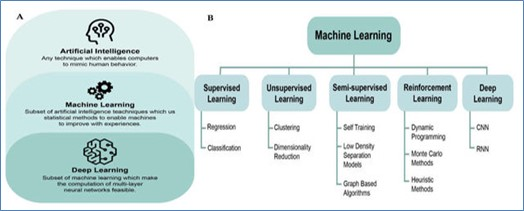
\includegraphics[width=1\columnwidth]{bab2/Gambar/Picture1.jpg}
	\end{center}
	\vspace{-0.2cm}
	%\rule{\columnwidth}{0.1pt}
	\caption{(a) Hubungan Artificial Intelligence, Machine Learning, dan Deep Learning. (b) Jenis Machine Learning\\(Sumber: )}\label{img:Hubungan-Artificial-Intelligence}
\end{figure}
%%%%%%%%%%%%%%%%%%%%%%%%%% GAMBAR %%%%%%%%%%%%%%%%%%%%%%%%%%%%%%

Disamping hal tersebut, \textit{artificial intelligence} (AI) memungkinkan untuk berfikir, dan salah satu bagian dari \textit{artificial intelligence} untuk dapat melihat, mengamati, dan memahami adalah komputer visi atau \textit{computer vision}. \textit{Computer vision} memungkinkan untuk komputer dan sistem memberikan informasi berarti dari gambar digital, dan visual input. 

\section{\textit{Object Detection}}
\hspace{1,2cm}\textit{Object detection} atau deteksi objek dianggap sebagai salah satu bidang penting dalam pembelajaran mendalam dan visi komputer. Deteksi objek telah ditentukan oleh banyak aplikasi dalam visi komputer, seperti pelacakan objek, pengambilan, dan pengawasan video. Deteksi objek adalah teknologi \textit{deep learning} dimana benda, manusia, bengunan, mobil, dapat dideteksi sebagai objek dalam gambar dan video (U. Arshad, 2021).

Deteksi objek untuk mengenali objek dengan kotak pembatas pada gambar, dimana dalam klasifikasi gambar, cukup mengkategorikan (mengklasifikasikan) objek pada gambar atau tidak dalam hal kemungkinan (\textit{probability}), seperti contoh pada Gambar \ref{img:Classification-Object-Detection}

%%%%%%%%%%%%%%%%%%%%%%%%%% GAMBAR %%%%%%%%%%%%%%%%%%%%%%%%%%%%%%
\begin{figure}[H]
	\vspace{-0.1cm}
	%\rule{\columnwidth}{0.1pt}
	\begin{center}
		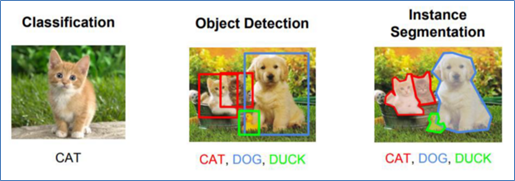
\includegraphics[width=1\columnwidth]{bab2/Gambar/Picture2.png}
	\end{center}
	\vspace{-0.2cm}
	%\rule{\columnwidth}{0.1pt}
	\caption{Classification, Object Detection dan Segmentation Representation\\(Sumber: A. Patel, 2020)}\label{img:Classification-Object-Detection}
\end{figure}
%%%%%%%%%%%%%%%%%%%%%%%%%% GAMBAR %%%%%%%%%%%%%%%%%%%%%%%%%%%%%%

Pada Gambar \ref{img:Segementation-Classification}, terlihat bahwa kucing (cat) dengan kotak pembatas dan tanpa kotak pembatas dapat membedakan mendasar antara klasifikasi citra dan deteksi objek.

%%%%%%%%%%%%%%%%%%%%%%%%%% GAMBAR %%%%%%%%%%%%%%%%%%%%%%%%%%%%%%
\begin{figure}[H]
	\vspace{-0.1cm}
	%\rule{\columnwidth}{0.1pt}
	\begin{center}
		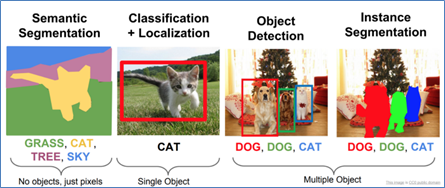
\includegraphics[width=1\columnwidth]{bab2/Gambar/Picture3.png}
	\end{center}
	\vspace{-0.2cm}
	%\rule{\columnwidth}{0.1pt}
	\caption{Segmentation, Classification+Localization, Object Detection\\(Sumber: \cite{Patel_2020})}\label{img:Segementation-Classification}
\end{figure}
%%%%%%%%%%%%%%%%%%%%%%%%%% GAMBAR %%%%%%%%%%%%%%%%%%%%%%%%%%%%%%

Dalam mempelajari deteksi objek, maka diperlukan mengetahui klasifikasi citra (\textit{image classification}). Ketika gambar adalah input ke CNN, masalah mengklasifikasikan kelas yang sesuai dengan gambar dikenal sebagai klasifikasi gambar, dan seperti yang ditunjukkan pada Gambar \ref{img:Image-Classification}, nilai probabilitas untuk semua kelas yang ditargetkan adalah keluaran.

%%%%%%%%%%%%%%%%%%%%%%%%%% GAMBAR %%%%%%%%%%%%%%%%%%%%%%%%%%%%%%
\begin{figure}[H]
	\vspace{-0.1cm}
	%\rule{\columnwidth}{0.1pt}
	\begin{center}
		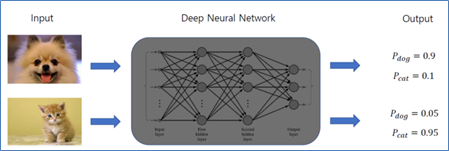
\includegraphics[width=1\columnwidth]{bab2/Gambar/Picture4.png}
	\end{center}
	\vspace{-0.2cm}
	%\rule{\columnwidth}{0.1pt}
	\caption{Image Classification\\(Sumber: A. Patel, 2020)}\label{img:Image-Classification}
\end{figure}
%%%%%%%%%%%%%%%%%%%%%%%%%% GAMBAR %%%%%%%%%%%%%%%%%%%%%%%%%%%%%%

Dapat juga dianggap bahwa deteksi objek sebagai masalah dimana tugas klasifikasi gambar memiliki tugas regresi yang memprediksi posisi objek menggunakan \textit{bounding box} (kotak pembatas) pada Gambar \ref{img:Object-Bounding-Box}. 

%%%%%%%%%%%%%%%%%%%%%%%%%% GAMBAR %%%%%%%%%%%%%%%%%%%%%%%%%%%%%%
\begin{figure}[H]
	\vspace{-0.1cm}
	%\rule{\columnwidth}{0.1pt}
	\begin{center}
		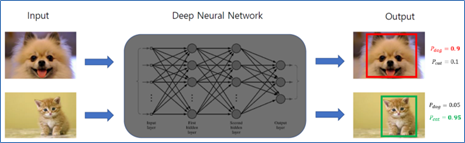
\includegraphics[width=1\columnwidth]{bab2/Gambar/Picture5.png}
	\end{center}
	\vspace{-0.2cm}
	%\rule{\columnwidth}{0.1pt}
	\caption{Object Detection dengan Bounding Box\\(Sumber: A. Patel, 2020)}\label{img:Object-Bounding-Box}
\end{figure}
%%%%%%%%%%%%%%%%%%%%%%%%%% GAMBAR %%%%%%%%%%%%%%%%%%%%%%%%%%%%%%

Masalah deteksi objek mengasumsikan bahwa beberapa kelas objek mungkin ada dalam gambar pada waktu yang sama. Dapat memvisualisasikan seperti dua jenis masalah, 1) klasifikasi multi label (beberapa kelas dalam satu gambar), 2) Bounding Box (masalah regresi) dimana harus memprediksi nilai koordinat kotak pembatas (\textit{bounding box}) dalam bentuk x, y, w, h.

Dalam deteksi objek, terdapat \textit{object localization} atau lokalisasi objek yang merupakan untuk memprediksi objek dalam sebuah citra serta batas-batasnya. Perbedaan antara lokalisasi objek dan deteksi objek tidak kentara. Sederhananya, lokalisasi objek bertujuan untuk menemukan objek utama (atau yang paling terlihat) dalam sebuah gambar, sedangkan deteksi objek mencoba untuk mengetahui semua objek dan batasannya.

Suatu klasifikasi citra atau model pengenalan citra hanya mendeteksi probabilitas suatu objek dalam suatu citra. Berbeda dengan ini, lokalisasi objek mengacu pada mengidentifikasi lokasi suatu objek dalam gambar. Algoritma lokalisasi objek akan menampilkan koordinat lokasi objek sehubungan dengan gambar. Dalam visi komputer, cara paling popular untuk melokalkan objek dalam gambar adalah dengan merepresentasikan lokasinya dengan bantuan kotak pembatas (\textit{bounding box}).

Bounding box dapat diinisialisasi menggunakan parameter berikut: 
\begin{itemize}
	\item bx, by: koordinat pusat kotak pembatas (center of bounding box)
	\item bw: lebar kotak pembatas dengan lebar gambar (width)
	\item bh: tinggi kotak pembatas dengan tinggi gambar (height)
\end{itemize}

%%%%%%%%%%%%%%%%%%%%%%%%%% GAMBAR %%%%%%%%%%%%%%%%%%%%%%%%%%%%%%
\begin{figure}[H]
	\vspace{-0.1cm}
	%\rule{\columnwidth}{0.1pt}
	\begin{center}
		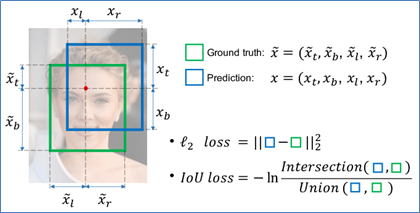
\includegraphics[width=1\columnwidth]{bab2/Gambar/Picture6.png}
	\end{center}
	\vspace{-0.2cm}
	%\rule{\columnwidth}{0.1pt}
	\caption{Intersection Over Union (IoU)\\(Sumber: A. Patel, 2020)}\label{img:Intersection-Over-Union}
\end{figure}
%%%%%%%%%%%%%%%%%%%%%%%%%% GAMBAR %%%%%%%%%%%%%%%%%%%%%%%%%%%%%%

Dengan memprediksi ini, dapat menghitung Mean-IoU dan memprediksi kotak pembatas (\textit{bounding box}) yang melokalkan objek di gambar.
\begin{itemize}
	\item IoU adalah Intersection-Over-Union (IoU) disebut sebagai Indeks Jaccard (\textit{Jaccard Index}) dianggap sebagai salah satu metrik kinerja yang paling banyak digunakan dalam deteksi objek. 

%%%%%%%%%%%%%%%%%%%%%%%%%% GAMBAR %%%%%%%%%%%%%%%%%%%%%%%%%%%%%%
\begin{figure}[H]
	\vspace{-0.1cm}
	%\rule{\columnwidth}{0.1pt}
	\begin{center}
		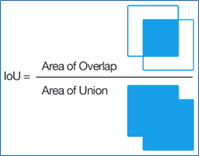
\includegraphics[width=0.4\columnwidth]{bab2/Gambar/Picture7.png}
	\end{center}
	\vspace{-0.2cm}
	%\rule{\columnwidth}{0.1pt}
	\caption{Persamaan IoU\\(Sumber: A. Patel, 2020)}\label{img:Persamaan-IOU}
\end{figure}
%%%%%%%%%%%%%%%%%%%%%%%%%% GAMBAR %%%%%%%%%%%%%%%%%%%%%%%%%%%%%%

	\item IoU adalah area tumpang tindih (\textit{overlap}) antara segmentasi yang diprediksi (\textit{prediction}) dan kebenaran dasar (\textit{ground truth}), seperti yang ditampilkan pada Gambar \ref{img:Persamaan-IOU}. Metrik ini bervariasi dari 0-1 (0-100\%) dengan 0 menyiratkan tidak ada tumpeng tindih (sampah) dan 1 menandakan segmentasi yang tumpang tindih sempurna (\textit{fat dub}).
	
	\item Mean IoU adalah segmentasi biner (dua kelas) atau multi-kelas, mean Io Udari gambar dihitung dengan mengambil IoU dari setiap kelas dan merata-ratakannya. 

\end{itemize}

\section{Machine Learning}
\hspace{1,2cm}Istilah \textit{machine learning} mula-mula diperkenalkan oleh Arthur Samuel pada tahun 1959 melalui jurnalnya yang berjudul "Some Studies in Machine Learning Using the Game of Checkers". (IBM Journal of Research and Development). Samuel mencoba mengajari program komputer untuk bermain catur. Tujuannya adalah membuat agar komputer dapat bermain catur lebih baik dari dirinya. Pada tahun 1962 program buatannya dapat mengalahkan juara catur dari negara bagian Connecticut (R. Primartha, 2018).

\textit{Machine learning} membutuhkan sebuah model yang didefinisikan berdasar parameter-parameter tertentu. Proses learning adalah eksekusi program komputer untuk mengoptimasi parameter-parameter dari model tersebut, dengan memanfaatkan data training atau \textit{past experience}.

Jadi, secara sederhana dapat dijelaskan bahwa \textit{machine learning} adalah pemrograman komputer untuk mencapai kriteria/performa tertentu dengan menggunakan sekumpulan data training atau pengalaman di masa lalu (\textit{past experience}). \textit{Machine learning} mempelajari teori agar komputer mampu "belajar" dari data. 

Secara umum algoritma \textit{machine learning} dapat dikelompokkan menjadi lima bagian, yaitu \textit{supervised learning}, \textit{unsupervised learning}, \textit{semi-supervised learning}, \textit{reinforcement learning}, dan \textit{deep learning}.

\subsection{Supervised Learning} 
\hspace{1,2cm}Sebagian besar praktik machine learning mengandalkan algoritma \textit{supervised learning}. Algoritmanya dinamakan seperti ini karena training dataset (sekumpulan data untuk training) akan memandu dan mengajari komputer agar menghasilkan outcome sesuai harapan. Pada \textit{supervised learning} menggunakan sebuah algoritma untuk mempelajari mapping function antara input dengan output. Berbagai kemungkinan output sudah diketahui dan data-data yang digunakan untuk latihan (training) sudah diberi label dengan jawaban yang benar. \textit{Supervised learning} dapat bermanfaat untuk memprediksi sesuatu dengan bantuan training dataset. Berikut skema \textit{supervised learning} pada Gambar \ref{img:Skema-Supervised-Learning} (R. Primartha, 2018).

%%%%%%%%%%%%%%%%%%%%%%%%%% GAMBAR %%%%%%%%%%%%%%%%%%%%%%%%%%%%%%
\begin{figure}[H]
	\vspace{-0.1cm}
	%\rule{\columnwidth}{0.1pt}
	\begin{center}
		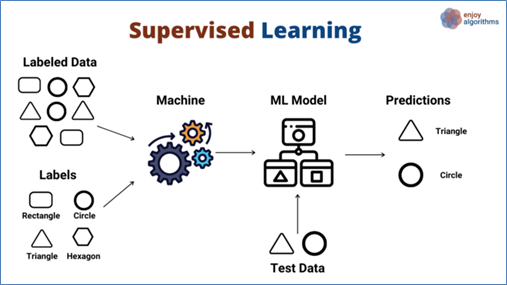
\includegraphics[width=1\columnwidth]{bab2/Gambar/Picture8.png}
	\end{center}
	\vspace{-0.2cm}
	%\rule{\columnwidth}{0.1pt}
	\caption{Skema Supervised Learning\\(Sumber: M. Kozan, 2021)}\label{img:Skema-Supervised-Learning}
\end{figure}
%%%%%%%%%%%%%%%%%%%%%%%%%% GAMBAR %%%%%%%%%%%%%%%%%%%%%%%%%%%%%%

\textit{Supervise learning} menggunakan training data yang sudah diberi label untuk mempelajari \textit{mapping function}, dari input variables (x) ke ouput variables (y).
\[y=f\ (x)\]

Sebagai contoh, sebuah algoritma klasifikasi akan dapat mengidentifikasi berbagai bentuk bangun setelah melalui proses belajar dari sekumpulan bangun datar yang sudah ditandai atau diberi label dengan ciri tertentu seperti pada gambar 2.12.

Permasalahan-permasalahan yang terkait dengan \textit{supervised learning} dapat dikategorikan menjadi dua jenis:
\begin{enumerate}
	\item \textit{Classification}
	
	Klasifikasi bertujuan untuk memprediksi outcome dari input (sample yang diberikan), dimana output variabel berbentuk kategori-kategori. Contoh: pria/wanita, sakit/sehat, tinggi/rendah, dan sebagainya.
	
	\item \textit{Regression}
	
	Regression bertujuan untuk memprediksi outcome dari input (sample yang diberikan), dimana output, variabel berbentuk nilai aktual (\textit{real values}). Contoh: prediksi harga rumah, tinggi badan seseorang, curah hujan, dan sebagainya. 
	
\end{enumerate}

Ada beberapa algoritma yang sudah dikembangkan dan terkait dengan \textit{supervised learning}, diantaranya:
\begin{enumerate}
	\item Decision tree,
	\item Naïve Bayes Classifier,
	\item Artificial Neural Network,
	\item Support Vector Machine,
	\item Linear Regression,
	\item Logistic Regression,
	\item CART,
	\item KNN (-KNearest Neighbor), dsb.
\end{enumerate}

\subsection{Unsupervised Learning}
\hspace{1,2cm}Berbeda dengan supervised learning, pada \textit{unsupervised learning} persoalan diproses hanya mengandalkan data yang belum dilatih sebelumnya. \textit{Unsepervised learning} menggunakan \textit{unlabeled training dataset} untuk memodelkan struktur dari data, sehingga unsupervised learning bersifat lebih subjektif dibandingkan \textit{supervised learning}. Berikut skema \textit{unsupervised learning} pada Gambar \ref{img:Skema-Unsupervised-Learning} (R. Primartha, 2018).

%%%%%%%%%%%%%%%%%%%%%%%%%% GAMBAR %%%%%%%%%%%%%%%%%%%%%%%%%%%%%%
\begin{figure}[H]
	\vspace{-0.1cm}
	%\rule{\columnwidth}{0.1pt}
	\begin{center}
		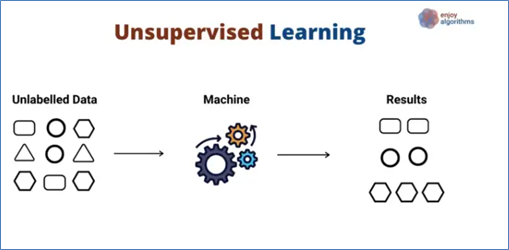
\includegraphics[width=1\columnwidth]{bab2/Gambar/Picture9.png}
	\end{center}
	\vspace{-0.2cm}
	%\rule{\columnwidth}{0.1pt}
	\caption{Skema Unsupervised Learning\\(Sumber: M. Kozan, 2021)}\label{img:Skema-Unsupervised-Learning}
\end{figure}
%%%%%%%%%%%%%%%%%%%%%%%%%% GAMBAR %%%%%%%%%%%%%%%%%%%%%%%%%%%%%%

\textit{Unsupervised learning} bermanfaat untuk kasus-kasus dimana kita ingin menemukan relasi implisit (implicit relationships) dari \textit{unlabeled dataset} yang disediakan. Jadi, pada \textit{unsupervised learning} kita tidak memprediksi masa depan, sebab input variable (X) tidak memiliki relasi dengan output variabel (Y). 
\[ f(x) \]

Untuk memudahkan memahaminya, dapat diasumsikan saat ini belum pernah membeli majalah sama sekali. Suatu ketika membeli beberapa buah majalah dan ingin membaginya menjadi beberapa kategori, dengan tujuan agar nantinya mudah dicari. Maka, dapat dimulai dengan mengidentifikasi majalah-majalah berdasarkan kemiripan. Misalnya, berdasarkan isi, penerbit, dan lain-lain yang bisa ditentukan sesuai kebutuhan.

Permasalahan seputar \textit{unsupervised learning} dapat dikelompokkan menjadi tiga kategori, yaitu:

\begin{enumerate}
	\item Association
	
	Association bertujuan untuk menemukan peluang (probabilitas) berdasarkan keterkaitan (co-occurrence) dari item-item dalam sebuah kumpulan. Sebuah contoh, jika customer membeli teh celup, maka kemungkinan besar (sekitar 80%) customer juga membeli gula pasir. Association banyak digunakan dalam market-basket analisis. 
	\item Clustering
	
	Clustering bertujuan untuk mengelompokkan sample dalam cluster yang sama berdasarkan kemiripan (similiarity).
	
	\item Dimensionality Reduction
	
	Dimensionality Reduction berarti mengurangi sejumlah variabel dari dataset namun tetap memastikan informasi yang penting masih tersedia. Dimensionality Reduction dapat diwujudkan menggunakan metode:
	\begin{enumerate}[label=(\alph*)]
		\item Feature Extraction
		
		Melakukan transformasi data dari dimensi tinggi (a high-dimensional space) ke dimensi yang lebih rendah (a low-dimensional space).
		
		\item Feature Selection
		
		Memilih Sebagian saja (subset) dari variabel asal (original variabel). 
	\end{enumerate}
\end{enumerate}

Beberapa algoritma yang dikelompokkan dalam \textit{unsupervised learning}, antara lain: 
\begin{enumerate}
	\item K-Means
	\item Hierarchical Clustering
	\item DBSCAN
	\item Fuzzy C-Means
	\item Self-Orginizing Map, dan sebagainya.	
	
\end{enumerate}

\subsection{Semi-supervised learning}
\hspace{1,2cm}Metode ini berada diantara yang \textit{supervised} dan \textit{unsupervised learning} di mana memiliki sejumlah besar masukan data, beberapa di antaranya diberi label dan sisanya tidak. Banyak masalah pembelajaran kehidupan nyata termasuk dalam bidang pembelajaran mesin ini. Alasannya adalah \textit{semi-supervised} membutuhkan lebih sedikit intervensi manusia karena menggunakan data berlabel dalam jumlah yang sangat kecil dan data yang tidak berlabel dalam jumlah besar. Memanfaatkan kumpulan data yang kurang berlabel lebih menarik karena kumpulan data tersebut sangat sulit untuk dikumpulkan serta mahal dan mungkin memerlukan akses ke pakar domain. Dataset yang tidak berlabel di sisi lain lebih murah dan lebih mudah diakses (X. Zhu, 2018).

Kedua teknik pembelajaran \textit{supervised} dan \textit{unsupervised learning} bisa digunakan untuk melatih algoritma pembelajaran dalam pembelajaran \textit{semi-supervised}. Teknik \textit{unsupervised learning} dapat digunakan untuk mengungkap struktur dan pola tersembunyi dalam kumpulan data input. Sedangkan teknik supervised learning dapat digunakan untuk membuat prediksi tebakan pada data yang tidak berlabel, memasukkan data kembali ke algoritma pembelajaran sebagai data pelatihan, dan menggunakan pengetahuan yang diperoleh untuk membuat prediksi pada kumpulan data baru. Dengan demikian, dapat mengatakan bahwa data yang tidak berlabel digunakan untuk memodifikasi atau memprioritaskan kembali prediksi atau hipotesis yang diperoleh dari data yang berlabel. Gambar \ref{img:Skema-Semi-Supervised-Learning} mengilustrasikan berbagai tahapan metode \textit{semi-supervised learning}.

%%%%%%%%%%%%%%%%%%%%%%%%%% GAMBAR %%%%%%%%%%%%%%%%%%%%%%%%%%%%%%
\begin{figure}[H]
	\vspace{-0.1cm}
	%\rule{\columnwidth}{0.1pt}
	\begin{center}
		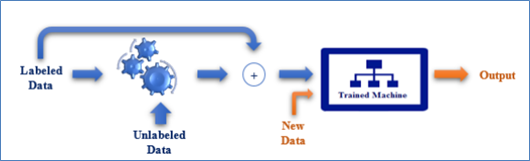
\includegraphics[width=1\columnwidth]{bab2/Gambar/Picture10.png}
	\end{center}
	\vspace{-0.2cm}
	%\rule{\columnwidth}{0.1pt}
	\captionsetup{justification=centering}
	\caption{Skema Semi-Supervised Learning\\(Sumber: )}\label{img:Skema-Semi-Supervised-Learning}
\end{figure}
%%%%%%%%%%%%%%%%%%%%%%%%%% GAMBAR %%%%%%%%%%%%%%%%%%%%%%%%%%%%%%

Untuk memanfaatkan data pelatihan yang tidak berlabel, semua algoritma \textit{semi-supervised learning} melakukan setidaknya satu dari asumsi berikut asumsi kehalusan, asumsi cluster, dan asumsi manifold.

\subsection{Reinforcement Learning}
\hspace{1,2cm}\textit{Reinforcement learning} merupakan metode pembelajaran yang dipengaruhi oleh feedback dari lingkungan dengan Teknik pembelajaran yang iterative (berulang-ulang) dan adaptive (menyesuaikan). \textit{Reinforcement learning} dipercaya mendekati cara manusia belajar (R. Primartha, 2018). 

\textit{Reinforcement learning} (RL) diinspirasi oleh kebiasaan makhluk hidup dalam belajar dan bertindak, khususnya manusia. Pada RL tidak ada dataset. Data-data diperoleh berdasarkan pengalaman. Algoritma \textit{reinforcement learning} mengijinkan agent untuk memutuskan aksi selanjutnya berdasarkan kondisi saat ini (\textit{current state}). \textit{Reinforcement learning} kadang disebut juga \textit{credit assessment learning}, sebab learning difokuskan untuk memaksimalkan perolehan \textit{rewards}. \textit{Reinforcement learning} tergantung pada proses coba-coba untuk mengungkap rangkaian tindakan yang memaksimalkan metrik imbalan kumulatif, yang digunakan untuk membuat algoritma memahami apakah itu mengarah ke arah yang benar atau tidak. Berikut skema \textit{reinforcement learning} pada Gambar \ref{img:Skema-Reinforcement-Learning}. 

%%%%%%%%%%%%%%%%%%%%%%%%%% GAMBAR %%%%%%%%%%%%%%%%%%%%%%%%%%%%%%
\begin{figure}[H]
	\vspace{-0.1cm}
	%\rule{\columnwidth}{0.1pt}
	\begin{center}
		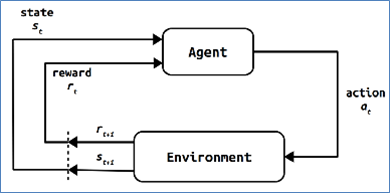
\includegraphics[width=1\columnwidth]{bab2/Gambar/Picture11.png}
	\end{center}
	\vspace{-0.2cm}
	%\rule{\columnwidth}{0.1pt}
	\captionsetup{justification=centering}
	\caption{Skema Reinforcement Learning\\(Sumber: R. Sutton, 1998)}\label{img:Skema-Reinforcement-Learning}
\end{figure}
%%%%%%%%%%%%%%%%%%%%%%%%%% GAMBAR %%%%%%%%%%%%%%%%%%%%%%%%%%%%%%

Menurut R. Sutton, proses \textit{reinforcement learning} dapat dipresentasikan dalam matematika sebagai \textit{Markov Decision Process} (MDP), memperkenalkan 4 set {S, A, P, R}, dengan:\\
S - Kumpulan status tempat agen dapat berada, pada saat tertentu;\\
A - Serangkaian kemungkinan Tindakan yang dapat dilakukan agen dalam waktu tertentu;\\
P - Himpunan probabilitas, bahwa sebuah agen, yang berada dalam keadaan s, bertransisi ke keadaan s' dengan melakukan Tindakan A dalam waktu t+1;

Representasi \textit{reinforcement learning} mirip dengan supervised learning. Yang membedakan adalah pada reinforcement learning tidak hanya x, namun x dan z.
\[ y=\ f\ \left(x\right)\ given\ z \]

Tidak seperti \textit{supervised} dan \textit{unsupervised learning} dimana algoritma sudah memiliki tujuan (goal). Algoritma \textit{reinforcement learning} tidak memiliki tujuan eksplisit, sebagai gantinya algoritma dipaksa untuk belajar menemukan nilai optimal melalui kegiatan trial dan error.

\textit{Reinforcement learning} banyak diimplementasikan pada \textit{game theory, control theory, operation research, information theory, simulation-based optimaztion, multi-agent systems, swarm intelligence, statistics}, dan \textit{genetic algorithm}.

Contoh penerapan \textit{reinforcement learning} yaitu pada bidang robotic. Sebuah robot dapat belajar untuk menghindari tabrakan dengan cara menerima feedback negative manakala robot tersebut menabrak halangan tertentu. Robot akan dibiarkan berjalan tanpa dipandu. Robot akan belajar dari pengalaman sebelumnya untuk menemukan rute paling optimal. 

Beberapa algoritma yang dikelompokkan dalam \textit{reinforcement learning} antara lain:
\begin{enumerate}
	\item Genetic Algorithm (GA)
	\item Dynamic Programming (DP)
	\item Generalized Policy Iteration (GPI)
	\item Monte Carlo Methods
\end{enumerate}

\subsection{Deep Learning}
\hspace{1,2cm}\textit{Deep learning} merupakan metode pembelajaran yang memanfaatkan \textit{artificial neural networks} yang berlapis-lapis (multi layer). \textit{Artificial neural networks} ini dibuat mirip dengan otak manusia, di mana neuron-neuron terkoneksi satu sama lain, sehingga membentuk sebuah jaringan neuron yang sangat rumit (R. Primartha, 2018).

\textit{Deep learning} atau \textit{deep structured leaning} atau hierarchical learning atau deep neural merupakan metode pembelajaran yang memanfaatkan multiple non-linear transformation. \textit{Deep learning} dapat dipandang sebagai gabungan machine learning dengan \textit{artificial intelligence} (AI). \textit{Deep learning} pada hakekatnya merupakan perluasan atau pengembangan dari \textit{neural network} atau jaringan saraf tiruan (JST).

Jika dikembalikan kepada tujuan \textit{machine learning} semula, yaitu komputer yang dapat belajar (dari data atau pengalaman), maka \textit{deep learning} adalah apa yang selama ini dicari. \textit{Deep learning} menirukan cara berpikir manusia. Pada \textit{deep learning}, komputer harus memproses data yang sangat banyak, berlapis-lapis, dan output dari layer sebelumnya akan menjadi input bagi layer sesudahnya.

Struktur umum dan dasar dari skema \textit{deep learning} ditunjukkan pada Gambar \ref{img:Skema-Umum-Deep-Learning}. Ini terdiri dari lapisan masukan, yang merupakan data masukan ke algoritma; lapisan tersembunyi, di mana algoritma membuat banyak perhitungan matematis, dan lapisan output, yang merupakan hasil dari perhitungan algoritma.

%%%%%%%%%%%%%%%%%%%%%%%%%% GAMBAR %%%%%%%%%%%%%%%%%%%%%%%%%%%%%%
\begin{figure}[H]
	\vspace{-0.1cm}
	%\rule{\columnwidth}{0.1pt}
	\begin{center}
		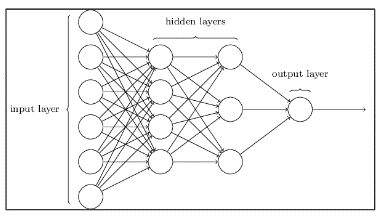
\includegraphics[width=1\columnwidth]{bab2/Gambar/Picture12.png}
	\end{center}
	\vspace{-0.2cm}
	%\rule{\columnwidth}{0.1pt}
	\captionsetup{justification=centering}
	\caption{Skema Umum \textit{Deep Learning}\\(Sumber: \citep{Feizollah2022-tn})}\label{img:Skema-Umum-Deep-Learning}
\end{figure}
%%%%%%%%%%%%%%%%%%%%%%%%%% GAMBAR %%%%%%%%%%%%%%%%%%%%%%%%%%%%%%
Sejarah \textit{deep learning} dimulai pada tahun 2006, yaitu setelah Geoffrey Hinton mempublikasikan paper yang memperkenalkan salah satu varian \textit{neural networks} yang disebut \textit{deep belief nets}. Paper ini merupakan awal kemunculan istilah \textit{deep learning}, untuk membedakan arsitektur \textit{neural network} konvensional (\textit{single layer}) dengan arsitektur neural network multi/banyak layer. Dengan kata lain, deep learning adalah salah satu cabang machine learning yang menggunakan \textit{deep neural network} untuk menyelesaikan permasalahan pada domain \textit{machine learning}. 

Pada tahun 2009, Andrew memperkenalkan penggunaan GPU untuk \textit{deep learning} melalui paper yang berjudul \textit{large-scale deep unsupervised learning using graphics processors}. Dengan menggunakan GPU, algoritma \textit{deep learning} dapat dijalankan lebih cepat disbanding dengan tanpa GPU (hanya menggunakan CPU), Perkembangan \textit{deep learning} maju pesat berkat keberadaan \textit{hardware} yang memadai. Dan saat ini, \textit{deep learning} sudah banyak diaplikasikan di berbagai area, seperti pengenal wajah, \textit{self-driving car}, pengenal suara, dan sebagainya. 

\textit{Deep learning} merupakan jalan untuk mencapai apa yang sudah dicita-citakan sebelumnya oleh manusia, yaitu kecerdasan buatan bagi mesin. Bentuk diagram \textit{network model deep learning} seperti pada Gambar \ref{img:Skema-Deep-Learning-Hidden-Layer}. Perhatikan bahwa \textit{hidden layer} hanya digambarkan tiga lapis saja, padahal kenyataanya bisa berjumlah sangat banyak, dapat diasumsikan seperti Gambar \ref{img:Skema-Deep-Learning-Hidden-Layer}.

%%%%%%%%%%%%%%%%%%%%%%%%%% GAMBAR %%%%%%%%%%%%%%%%%%%%%%%%%%%%%%
\begin{figure}[H]
	\vspace{-0.1cm}
	%\rule{\columnwidth}{0.1pt}
	\begin{center}
		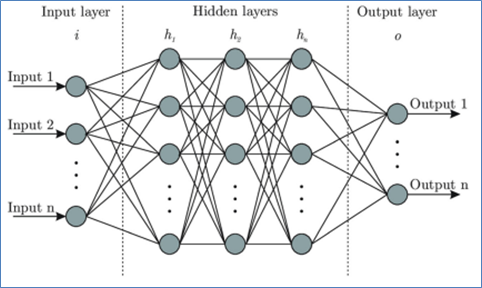
\includegraphics[width=1\columnwidth]{bab2/Gambar/Picture13.png}
	\end{center}
	\vspace{-0.2cm}
	%\rule{\columnwidth}{0.1pt}
	\captionsetup{justification=centering}
	\caption{Skema \textit{Deep Learning} dengan Penambahan beberapa \textit{hidden layer}\\(Sumber: H. Kaur et al, 2021)}\label{img:Skema-Deep-Learning-Hidden-Layer}
\end{figure}
%%%%%%%%%%%%%%%%%%%%%%%%%% GAMBAR %%%%%%%%%%%%%%%%%%%%%%%%%%%%%%

Pada Gambar \ref{img:Skema-Deep-Learning-Hidden-Layer} mengandung 3 layer, yaitu input, \textit{hidden} dan output layer. Penambahan \textit{layer} ini terjadi pada \textit{hidden layer}. \textit{Hidden layer} pada skema \textit{deep learning} yang disebut dengan \textit{Multi Layer Peceptron} (MLP) disebabkan jumlah neuron semakin banyak dan itu artinya semakin banyak juga perhitungan yang harus dikerjakan pada setiap \textit{layer}. MLP merupakan pengembangan dari \textit{Single Layer Perceptron} (SLP) yang merupakan model paling sederhana dari neural network dan sekaligus merupakan dasar bagi model-model tingkat lanjut yang digunakan pada \textit{deep learning}. MLP kemudian menjadi cikal bakal metode \textit{deep learning} atau \textit{deep neural network} (DNN).

\textit{Deep learning} sudah dikembangkan ke berbagai model atau arsitektur yang berbeda-beda. Berikut daftar beberapa model atau arsitektur untuk \textit{deep learning}. 
\begin{enumerate}
	\item \textit{Recurrent Neural Networks} (RNN)
	\item \textit{Long Short-Term Memory} (LSTM)
	\item \textit{Convolutional Neural Network} (CNN)
	\item \textit{Deep Believe Networks} (DBN)
	\item \textit{Deep Stacking Networks} (DSN)
\end{enumerate}

Contoh penerapan masing-masing arsitektur deep learning dapat dipelajari pada Tabel \ref{tbl:Penerapan-Arsitektur-Deep-Learning}
%%%%%%%%%%%%%%%%%%%%%%%TABEL SEDERHANA%%%%%%%%%%%%%%%%%%%%%%%%%
\begin{singlespace}
	\begin{table}[H]
		\centering
		\caption{Penerapan Arsitektur Deep Learning}
		\label{tbl:Penerapan-Arsitektur-Deep-Learning}
		\begin{adjustbox}{width=\columnwidth,center}
			\begin{tabular}{|c|c|l|}
				\hline
				No. & Arsitektur & \multicolumn{1}{c|}{Penerapan}                                                                                                                                           \\ \hline
				1   & RNN        & \textit{Speech recognition, handwriting recognition}                                                                                                                     \\ \hline
				2   & LSTM       & \textit{\begin{tabular}[c]{@{}l@{}}Natural language text compression, handwriting recognition,\\ speech recognition, gesture recognition, image captioning\end{tabular}} \\ \hline
				3   & CNN        & \textit{Image recognition, video analysis, natural language processing}                                                                                                  \\ \hline
				4   & DBN        & \textit{\begin{tabular}[c]{@{}l@{}}Image recognition, information retrieval, \\ natural language understanding, failure prediction\end{tabular}}                         \\ \hline
				5   & DSN        & \textit{Information retrieval, continuous speech recognition}                                                                                                            \\ \hline
			\end{tabular}
		\end{adjustbox}
	\end{table}
\end{singlespace}
%%%%%%%%%%%%%%%%%%%%%%%TABEL SEDERHANA%%%%%%%%%%%%%%%%%%%%%%%%%
Masing-masing arsitektur pada Tabel \ref{tbl:Penerapan-Arsitektur-Deep-Learning} memiliki perbedaan, berikut penjelasan dan diagram network beberapa arsitektur deep learning yang umum.

\subsubsection{Recurrent Neural Networks (RNN)}
\hspace{1,2cm}\textit{Recurrent Neural Network} (RNN) merupakan arsitektur \textit{deep learning} yang popular serta sangat menjanjinak untuk menyelesaikan berbagai persoalan yang terkait dengan \textit{Natural Language Processing} (NLP). Model RNN digunakan agar mesin dapat memahami bahasa manusia. Mulai dari cara berkomunikasi, mendengarkan, mengenali percakapan, hingga memahami tata bahasa dan aksen. RNN juga dapat diimplementasikan untuk mengenali gambar-gambar atau objek (R. Primartha, 2018).

Diagram network RNN seperti pada Gambar \ref{img:Diagram-RNN} berikut. 
%%%%%%%%%%%%%%%%%%%%%%%%%% GAMBAR %%%%%%%%%%%%%%%%%%%%%%%%%%%%%%
\begin{figure}[H]
	\vspace{-0.1cm}
	%\rule{\columnwidth}{0.1pt}
	\begin{center}
		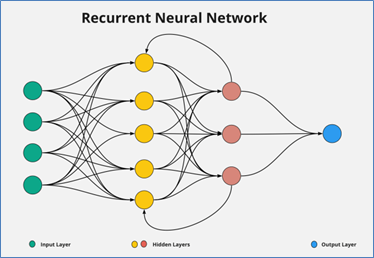
\includegraphics[width=0.8\columnwidth]{bab2/Gambar/Picture14.png}
	\end{center}
	\vspace{-0.2cm}
	%\rule{\columnwidth}{0.1pt}
	\captionsetup{justification=centering}
	\caption{Diagram \textit{Recurent Neural Network} (RNN)\\(Sumber: K. Dass, 2020)}\label{img:Diagram-RNN}
\end{figure}
%%%%%%%%%%%%%%%%%%%%%%%%%% GAMBAR %%%%%%%%%%%%%%%%%%%%%%%%%%%%%%

\subsubsection{Long Short Term Memory (LSTM)}
\hspace{1,2cm}\textit{Long Short Term Memory} (LSTM) merupakan building unit untuk \textit{layer-layer} pada recurrent neural network (RNN). LSTM mula-mula diusulkan oleh Sepp Hochreiter dan Jurgen Schmidhuber pada tahun 1997. LSTM juga banyak diimplementasikan pada bidang NLP. Boleh dibilang LSTM merupakan pengembangan dari RNN. Secara teoritis, jaringan saraf yang terhubung secara naif, yang disebut jaringan saraf berulang, dapat bekerja. Namun dalam praktiknya, mengalami dua masalah: gradien menghilang dan gradien meledak, yang membuatnya tidak dapat digunakan (R. Primartha, 2018).  Kemudian, LSTM ditemukan untuk mengatasi masalah ini dengan secara eksplisit memasukkan unit memori, yang disebut sel ke dalam jaringan. Ini adalah diagram blok bangunan LSTM pada Gambar \ref{img:Diagram-LSTM}.

%%%%%%%%%%%%%%%%%%%%%%%%%% GAMBAR %%%%%%%%%%%%%%%%%%%%%%%%%%%%%%
\begin{figure}[H]
	\vspace{-0.1cm}
	%\rule{\columnwidth}{0.1pt}
	\begin{center}
		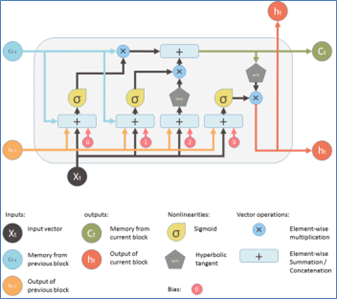
\includegraphics[width=0.8\columnwidth]{bab2/Gambar/Picture15.png}
	\end{center}
	\vspace{-0.2cm}
	%\rule{\columnwidth}{0.1pt}
	\captionsetup{justification=centering}
	\caption{Diagram \textit{Long Short Term Memory} (LSTM) \\(Sumber: S. Yan, 2016)}\label{img:Diagram-LSTM}
\end{figure}
%%%%%%%%%%%%%%%%%%%%%%%%%% GAMBAR %%%%%%%%%%%%%%%%%%%%%%%%%%%%%%

\subsubsection{Convolutional Neural Network (CNN)}
\hspace{1,2cm}\textit{Convolutional Neural Networks} (CNN atau ConvNet) merupakan salah satu model deep learning yang banyak digunakan untuk keperluan analisis citra/visual. CNN adalah salah satu kategori utama untuk melakukan pengenalan dan klasifikasi gambar, deteksi objek, pengenalan wajah, dan sebagainya merupakan beberapa area dimana CNN banyak digunakan (R. Primartha, 2018).

Klasifikasi gambar CNN mengambil input gambar, memproses, dan mengklasifikasikannya dalam kategori tertentu, misalnya kucing, harimau, singa. Komputer melihat gambar input sebagai susunan piksel dan itu tergantung pada resolusi gambar. Berdasarkan resolusi gambar, akan terlihat h x w x d (h = Tinggi, w = Lebar, d = Dimensi). Misalnya, gambar array matriks RGB 6 x 6 x 3 (3 mengacu pada nilai RGB) dan gambar array matriks 4 x 4 x 1 dari gambar skala abu-abu, seperti pada Gambar \ref{img:Array-Matriks-RGB}.

%%%%%%%%%%%%%%%%%%%%%%%%%% GAMBAR %%%%%%%%%%%%%%%%%%%%%%%%%%%%%%
\begin{figure}[H]
	\vspace{-0.1cm}
	%\rule{\columnwidth}{0.1pt}
	\begin{center}
		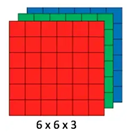
\includegraphics[width=0.3\columnwidth]{bab2/Gambar/Picture16.png}
	\end{center}
	\vspace{-0.2cm}
	%\rule{\columnwidth}{0.1pt}
	\captionsetup{justification=centering}
	\caption{Array dari Matriks RGB\\(Sumber: R. Prabhu, 2018)}\label{img:Array-Matriks-RGB}
\end{figure}
%%%%%%%%%%%%%%%%%%%%%%%%%% GAMBAR %%%%%%%%%%%%%%%%%%%%%%%%%%%%%%

Secara teknis, model \textit{deep learning} CNN untuk latih dan uji, setiap gambar input akan melewati serangkaian lapisan konvolusi dengan filter (Kernel), Pooling, \textit{fully connected layers} (FC) dan menerapkan fungsi softmax untuk mengklasifikasikan objek dengan nilai probabilistic antara 0 dan 1. Gambar 2.17. adalah alur dari CNN untuk memproses gambar input dan mengklasifikasikan objek berdasarkan nilai.


%%%%%%%%%%%%%%%%%%%%%%%%%% GAMBAR %%%%%%%%%%%%%%%%%%%%%%%%%%%%%%
\begin{figure}[H]
	\vspace{-0.1cm}
	%\rule{\columnwidth}{0.1pt}
	\begin{center}
		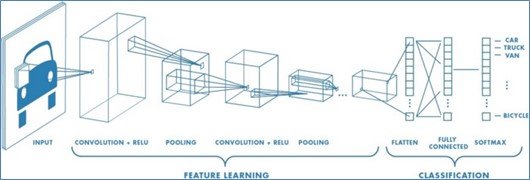
\includegraphics[width=1\columnwidth]{bab2/Gambar/Picture17.jpg}
	\end{center}
	\vspace{-0.2cm}
	%\rule{\columnwidth}{0.1pt}
	\captionsetup{justification=centering}
	\caption{Neural Network dengan banyak Convolusi Layer\\(Sumber: R. Prabhu, 2018)}\label{img:Neural-Network-Dengan-Banyak-Convolusi-Layer}
\end{figure}
%%%%%%%%%%%%%%%%%%%%%%%%%% GAMBAR %%%%%%%%%%%%%%%%%%%%%%%%%%%%%%

\begin{enumerate}
	\item \textit{Convolution Layer}
	
	Konvolusi adalah lapisan pertama untuk mengekstraksi fitur dari gambar masukan. Konvolusi mempertahankan hubungan antara piksel dengan mempelajari fitur gambar menggunakan kotak kecil data masukan. Ini adalah operasi matematika yang mengambil dua input, seperti matriks gambar dan filter atau kernel.
	
	\begin{itemize}
		\item Sebuah gambar matriks (volume) dari dimensi \textbf{(h x w x d)}
		\item Sebuah filter \textbf{(fh x fw x d)}
		\item Output volume dimensi \textbf{(h - fh + 1) x (w - fw + 1) x 1 }
		
		%%%%%%%%%%%%%%%%%%%%%%%%%% GAMBAR %%%%%%%%%%%%%%%%%%%%%%%%%%%%%%
		\begin{figure}[H]
			\vspace{-0.1cm}
			%\rule{\columnwidth}{0.1pt}
			\begin{center}
				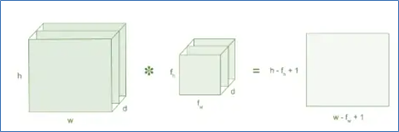
\includegraphics[width=1\columnwidth]{bab2/Gambar/Picture18.png}
			\end{center}
			\vspace{-0.2cm}
			%\rule{\columnwidth}{0.1pt}
			\captionsetup{justification=centering}
			\caption{Gambar Matriks Multiplies Kernel atau Filter Matriks\\(Sumber: R. Prabhu, 2018)}\label{img:Matriks-Multiplies}
		\end{figure}
		%%%%%%%%%%%%%%%%%%%%%%%%%% GAMBAR %%%%%%%%%%%%%%%%%%%%%%%%%%%%%%
	\end{itemize}
	Pertimbangkan gambar 5 x 5 yang nilai piksel gambarnya adalah 0, 1 dan matriks filter 3 x 3, seperti pada Gambar \ref{img:Matriks5x5}.
	
	%%%%%%%%%%%%%%%%%%%%%%%%%% GAMBAR %%%%%%%%%%%%%%%%%%%%%%%%%%%%%%
	\begin{figure}[H]
		\vspace{-0.1cm}
		%\rule{\columnwidth}{0.1pt}
		\begin{center}
			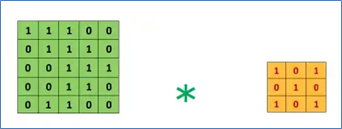
\includegraphics[width=0.7\columnwidth]{bab2/Gambar/Picture19.png}
		\end{center}
		\vspace{-0.2cm}
		%\rule{\columnwidth}{0.1pt}
		\captionsetup{justification=centering}
		\caption{Gambar matriks 5 x 5 dikalikan dengan Filter matiks 3 x 3}\label{img:Matriks5x5}
	\end{figure}
	%%%%%%%%%%%%%%%%%%%%%%%%%% GAMBAR %%%%%%%%%%%%%%%%%%%%%%%%%%%%%% 
	
	Kemudian, konvolusi matriks gambar 5 x 5 dikalikan dengan filter matriks 3 x 3 yang disebut "Feature Map" sebagai output yang ditunjukkan pada Gambar \ref{img:Output-Matriks-3-3}.
	
	%%%%%%%%%%%%%%%%%%%%%%%%%% GAMBAR %%%%%%%%%%%%%%%%%%%%%%%%%%%%%%
	\begin{figure}[H]
		\vspace{-0.1cm}
		%\rule{\columnwidth}{0.1pt}
		\begin{center}
			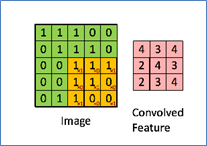
\includegraphics[width=0.7\columnwidth]{bab2/Gambar/Picture20.png}
		\end{center}
		\vspace{-0.2cm}
		%\rule{\columnwidth}{0.1pt}
		\captionsetup{justification=centering}
		\caption{Output Matriks 3 x 3}\label{img:Output-Matriks-3-3}
	\end{figure}
	%%%%%%%%%%%%%%%%%%%%%%%%%% GAMBAR %%%%%%%%%%%%%%%%%%%%%%%%%%%%%%
	
	Konvolusi gambar dengan filter berbeda dapat melakukan operasi seperti deteksi tepi, mengaburkan, dan memeprtajam dengan menerapkan filter. Berikut ini contoh yang menunjukkan berbagai gambar konvolusi setelah menerapkan berbagai jenis filter (Kernel) pada Gambar \ref{img:Fitur-Umum}.
	
	%%%%%%%%%%%%%%%%%%%%%%%%%% GAMBAR %%%%%%%%%%%%%%%%%%%%%%%%%%%%%%
	\begin{figure}[H]
		\vspace{-0.1cm}
		%\rule{\columnwidth}{0.1pt}
		\begin{center}
			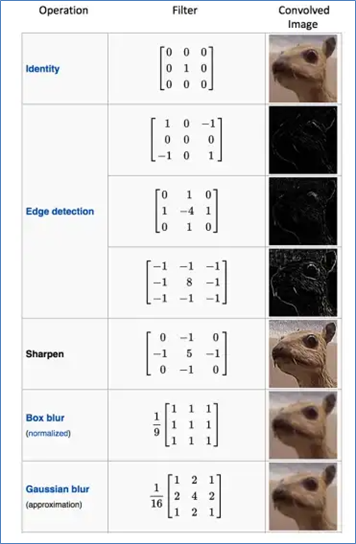
\includegraphics[width=0.6\columnwidth]{bab2/Gambar/Picture21.png}
		\end{center}
		\vspace{-0.2cm}
		%\rule{\columnwidth}{0.1pt}
		\captionsetup{justification=centering}
		\caption{Beberapa Filter Umum\\(Sumber: R. Prabhu, 2018)}\label{img:Fitur-Umum}
	\end{figure}
	%%%%%%%%%%%%%%%%%%%%%%%%%% GAMBAR %%%%%%%%%%%%%%%%%%%%%%%%%%%%%%
	
	\item Strides
	
	Stride adalah jumlah piksel yang bergeser di atas matriks input. Saat langkahnya 1, maka memindahkan filter ke 1 piksel sekaligus. Saat langkahnya 2, maka memindahkan filter ke 2 piksel sekaligus dan seterusnya. Gambar \ref{img:Stride-2-Piksel} menunjukkan konvolusi akan bekerja dengan Langkah 2.
	
	%%%%%%%%%%%%%%%%%%%%%%%%%% GAMBAR %%%%%%%%%%%%%%%%%%%%%%%%%%%%%%
	\begin{figure}[H]
		\vspace{-0.1cm}
		%\rule{\columnwidth}{0.1pt}
		\begin{center}
			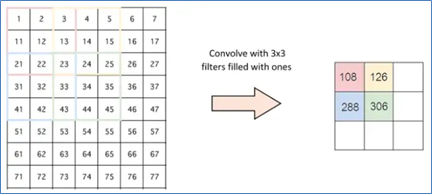
\includegraphics[width=0.6\columnwidth]{bab2/Gambar/Picture22.png}
		\end{center}
		\vspace{-0.2cm}
		%\rule{\columnwidth}{0.1pt}
		\captionsetup{justification=centering}
		\caption{Stride 2 Piksel\\(Sumber: R. Prabhu, 2018)}\label{img:Stride-2-Piksel}
	\end{figure}
	%%%%%%%%%%%%%%%%%%%%%%%%%% GAMBAR %%%%%%%%%%%%%%%%%%%%%%%%%%%%%%
	
	\item Padding
	
	Pada saat penggunaan filter, terkadang filter tidak pas dengan gambar masukan. Maka, terdapat dua pilihan: 
	\begin{itemize}
		\item Memadatkan gambar dengan angka nol (\textit{zero padding}) agar pas; 
		\item Menghilangkan bagian gambar yang tidak sesuai dengan filter. Ini disebut dengan \textit{valid padding} yang hanya menyimpan bagian gambar yang valid. 
		
	\end{itemize}
	
	\item Non Linerarity (ReLU)
	
	ReLU adalah singkatan dari \textit{Rectified Linear Unit} untuk operasi non-linear. Outputnya adalah \textit{f(x) = maks(0,x)}. ReLU penting karena tujuan ReLU adalah untuk mengenalkan non-linearitas di ConvNet, karena data dunia nyata ingin ConvNet pelajari adalah nilai linier non-negatif. Fungsi ini hanya mengembalikan nilai 0 jika nilai tersebut bernilai negative, selain itu mengembalikan nilai yang sama dengan yang diberikan, tidak lain adalah menghilangkan keluaran negative dan mempertahankan nilai antara 0 hingga + tak terhingga, seperti pada Gambar \ref{img:Operasi-RELU}. 
	
	%%%%%%%%%%%%%%%%%%%%%%%%%% GAMBAR %%%%%%%%%%%%%%%%%%%%%%%%%%%%%%
	\begin{figure}[H]
		\vspace{-0.1cm}
		%\rule{\columnwidth}{0.1pt}
		\begin{center}
			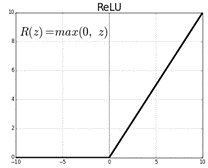
\includegraphics[width=0.3\columnwidth]{bab2/Gambar/Picture23.1.png}\\
			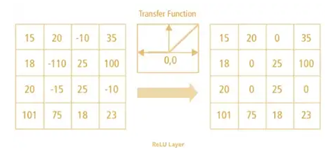
\includegraphics[width=0.6\columnwidth]{bab2/Gambar/Picture23.2.png}
		\end{center}
		\vspace{-0.2cm}
		%\rule{\columnwidth}{0.1pt}
		\captionsetup{justification=centering}
		\caption{Operasi ReLU\\(Sumber: P. Ratan, 2021)}\label{img:Operasi-RELU}
	\end{figure}
	%%%%%%%%%%%%%%%%%%%%%%%%%% GAMBAR %%%%%%%%%%%%%%%%%%%%%%%%%%%%%%
	
	\item Pooling Layer
	
	Bagian layer pooling akan mengurangi jumlah parameter ketika gambar terlalu besar. Penyatuan spasial juga disebut subsampling atau downsampling yang mengurangi dimensi setiap peta tetapi tetap mempertahankan informasi penting. Penyatuan spasial dapat dari berbagai jenis, diantaranya Max Pooling, Average Pooling, dan Sum Pooling.\\
	Max Pooling mengambil elemen tersbesar dari peta fitur yang diperbaiki. Mengambil elemen terbesar juga bisa mengambil pooling rata-rata. Jumlah semua elemen dalam peta fitur disebut sebagai kumpulan jumlah.
	
	%%%%%%%%%%%%%%%%%%%%%%%%%% GAMBAR %%%%%%%%%%%%%%%%%%%%%%%%%%%%%%
	\begin{figure}[H]
		\vspace{-0.1cm}
		%\rule{\columnwidth}{0.1pt}
		\begin{center}
			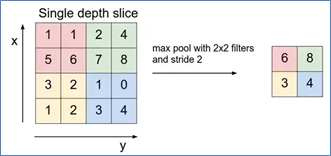
\includegraphics[width=0.5\columnwidth]{bab2/Gambar/Picture24.png}
		\end{center}
		\vspace{-0.2cm}
		%\rule{\columnwidth}{0.1pt}
		\captionsetup{justification=centering}
		\caption{Max Pooling}\label{img:Max-Polling}
	\end{figure}
	%%%%%%%%%%%%%%%%%%%%%%%%%% GAMBAR %%%%%%%%%%%%%%%%%%%%%%%%%%%%%%
	
	\item Fully Connected Layer

	Lapisan yang disebut \textit{Fully Connected Layer}, diratakan matriks menjadi vector dan memasukkannya ke dalam \textit{fully connected layer}, seperti jaringan saraf (\textit{neural network}), seperti Gambar \ref{img:Setelah-Pooling-Layer}.
	
	%%%%%%%%%%%%%%%%%%%%%%%%%% GAMBAR %%%%%%%%%%%%%%%%%%%%%%%%%%%%%%
	\begin{figure}[H]
		\vspace{-0.1cm}
		%\rule{\columnwidth}{0.1pt}
		\begin{center}
			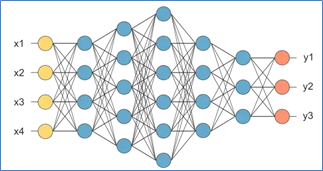
\includegraphics[width=0.5\columnwidth]{bab2/Gambar/Picture25.png}
		\end{center}
		\vspace{-0.2cm}
		%\rule{\columnwidth}{0.1pt}
		\captionsetup{justification=centering}
		\caption{Setelah Pooling Layer Diratakan sebagai FC Layer}\label{img:Setelah-Pooling-Layer}
	\end{figure}
	%%%%%%%%%%%%%%%%%%%%%%%%%% GAMBAR %%%%%%%%%%%%%%%%%%%%%%%%%%%%%%
	
	Pada Gambar \ref{img:Setelah-Pooling-Layer}, matriks peta fitur akan diubah menjadi vector (x1, x2, x3, ...). Dengan lapisan yang terhubung sepenuhnya, digabungkan fitur ini bersama untuk membuat model. Setelah itu, akhirnya memiliki fungsi aktivasi seperti softmax atau sigmoid untuk mengklasifikasikan keluaran sebagai objek, misalnya rumah, pohon, kucing, mobil, truk, dan sebagainya, seperti pada Gambar \ref{img:Arsitektur-CNN-Lengkap}.
	
	%%%%%%%%%%%%%%%%%%%%%%%%%% GAMBAR %%%%%%%%%%%%%%%%%%%%%%%%%%%%%%
	\begin{figure}[H]
		\vspace{-0.1cm}
		%\rule{\columnwidth}{0.1pt}
		\begin{center}
			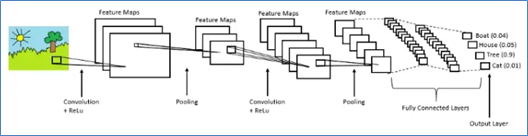
\includegraphics[width=0.5\columnwidth]{bab2/Gambar/Picture26.png}
		\end{center}
		\vspace{-0.2cm}
		%\rule{\columnwidth}{0.1pt}
		\captionsetup{justification=centering}
		\caption{Arsitektur CNN Lengkap}\label{img:Arsitektur-CNN-Lengkap}
	\end{figure}
	%%%%%%%%%%%%%%%%%%%%%%%%%% GAMBAR %%%%%%%%%%%%%%%%%%%%%%%%%%%%%%
	
\end{enumerate}

\subsubsection{Deep Believe Networks (DBN)}
\hspace{1,2cm}\textit{Deep Belief Neworks} (DBN) merupakan model \textit{deep learning} yang memanfaatkan tumpukan/\textit{stack Restricted Boltzmann Machines} (RBM) atau kadangkala \textit{Autoencoders}. \textit{Autoencoders} adalah model \textit{neural networks} yang memiliki input dan output yang sama. \textit{Autoencoder} mempelajari data input dan berusaha untuk melakukan rekonstruksi terhadap data input tersebut (R. Primartha, 2018).  Skema diagram DBN seperti pada Gambar \ref{img:Skema-Diagram-DBN}.

%%%%%%%%%%%%%%%%%%%%%%%%%% GAMBAR %%%%%%%%%%%%%%%%%%%%%%%%%%%%%%
\begin{figure}[H]
	\vspace{-0.1cm}
	%\rule{\columnwidth}{0.1pt}
	\begin{center}
		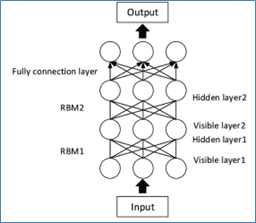
\includegraphics[width=0.6\columnwidth]{bab2/Gambar/Picture27.png}
	\end{center}
	\vspace{-0.2cm}
	%\rule{\columnwidth}{0.1pt}
	\captionsetup{justification=centering}
	\caption{Skema Diagram DBN\\(Sumber: H. Liu {\&} B. Lang, 2019)}\label{img:Skema-Diagram-DBN}
\end{figure}
%%%%%%%%%%%%%%%%%%%%%%%%%% GAMBAR %%%%%%%%%%%%%%%%%%%%%%%%%%%%%%

\subsubsection{Deep Stacking Networks (DSN)}
\hspace{1,2cm}Salah satu masalah pada \textit{deep learning} adalah proses learning sangat sulit dilakukan dan memerlukan komputasi yang cukup kompleks. Pada tahun 2011 Deng Yu mengusulkan model \textit{Deep Convex Networks} (DCN) atau \textit{Deep Stacking Network} (DSN), yang sedikit berbeda dibandingkan model \textit{deep learning} lain (R. Primartha, 2018). Secara umum model DSN terdiri atas ub-nets berukuran kecil dengan hanya sebuah hidden layer, seperti pada Gambar \ref{img:Skema-Diagram-DSN}.

%%%%%%%%%%%%%%%%%%%%%%%%%% GAMBAR %%%%%%%%%%%%%%%%%%%%%%%%%%%%%%
\begin{figure}[H]
	\vspace{-0.1cm}
	%\rule{\columnwidth}{0.1pt}
	\begin{center}
		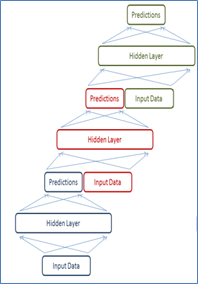
\includegraphics[width=0.4\columnwidth]{bab2/Gambar/Picture28.png}
	\end{center}
	\vspace{-0.2cm}
	%\rule{\columnwidth}{0.1pt}
	\captionsetup{justification=centering}
	\caption{Skema Diagram DSN\\(Sumber: L. Deng et al, 2012)}\label{img:Skema-Diagram-DSN}
\end{figure}
%%%%%%%%%%%%%%%%%%%%%%%%%% GAMBAR %%%%%%%%%%%%%%%%%%%%%%%%%%%%%%

Model \textit{deep learning} yang popular lainny aiatu Region Based CNN, Google Net, Generative Adversarial Network (GAN), dan You Only Look Once (YOLO).

\section{You Only Look Once (YOLO)}
\hspace{1,2cm}\textit{You Only Look Once} (YOLO) adalah algoritma deteksi objek real-time yang diperkenalkan pada tahun 2015 oleh Joseph Redmon, Santosh Divvala, Rosh Girshick dan Ali Farhadi dalam paper dengan judul "You Only Look Once: Unified, Real-Time Object Detection" (J. Redmon et al., 2015). Penulis membingkai masalah deteksi objek sebagai masalah regresi tugas klasifikasi dengan memisahkan kotak pembatas (\textit{bounding box}) secara spasial dan menghubungkan probabilitas ke masing-masing gambar yang terdeteksi menggunakan \textit{convolutional neural network} (CNN). YOLO adalah \textit{Convolutional Neural Network} (CNN) untuk melakukan deteksi objek secara real-time (V. Meel, 2022) (G. Boesch, 2022).

Beberapa alasan mengapa YOLO baik digunakan untuk deteksi objek real-time, diantaranya:
\begin{enumerate}
	\item Kecepatan (\textit{speed})
	
	YOLO sangat cepat karena tidak berurusan dengan jalur pipa (\textit{pipelines}) yang rumit. YOLO dapat memproses gambar pada 45 frames per second (FPS). Selain itu, YOLO mencapai rata-rata presisi atau mean average precision (mAP) lebih dari dua kali dibandingkan dengan sistem real-time lainnya, yang menjadikannya kandidat yang bagus untuk pemrosesan real-time. Dari grafik pada Gambar \ref{img:Kecepatan-YOLO} diamati bahwa YOLO jauh melampaui pendeteksi objek lainnya dengan 91 FPS.
	
	%%%%%%%%%%%%%%%%%%%%%%%%%% GAMBAR %%%%%%%%%%%%%%%%%%%%%%%%%%%%%%
	\begin{figure}[H]
		\vspace{-0.1cm}
		%\rule{\columnwidth}{0.1pt}
		\begin{center}
			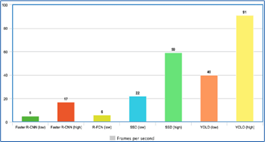
\includegraphics[width=0.4\columnwidth]{bab2/Gambar/Picture29.png}
		\end{center}
		\vspace{-0.2cm}
		%\rule{\columnwidth}{0.1pt}
		\captionsetup{justification=centering}
		\caption{Kecepatan YOLO dibandingkan dengan detector Objek Lainnya\\(Sumber: S. A. S. Hernandez et al, 2020)}\label{img:Kecepatan-YOLO}
	\end{figure}
	%%%%%%%%%%%%%%%%%%%%%%%%%% GAMBAR %%%%%%%%%%%%%%%%%%%%%%%%%%%%%%
	
	\item Akurasi deteksi tinggi (\textit{high detection accuracy})
	
	YOLO jauh melampaui model \textit{state-of-the-art} dalam akurasi dengan sedikit kesalahan latar belakang. 
	
	\item Generalisasi yang bagus (\textit{good generalization})
	
	YOLO mendorong sedikit lebih jauh dengan memberikan generalisasi yang lebih baik untuk domain baru, yang menjadikannya bagus untuk aplikasi yang mengandalkan deteksi objek yang cepat dan kuat. 
	
	\item Sumber terbuka (\textit{open-source})
	
	Membuat YOLO open-source membuat komunitas terus meningkatkan model. Inilah salah satu alasan mengapa YOLO telah melakukan begitu banyak perbaikan dalam waktu yang begitu terbatas. 
	
\end{enumerate}

\subsection{Arsitektur YOLO}
\hspace{1,2cm}Arsitektur YOLO memiliki keseluruhan 24 lapisan konvolusional, empat lapisan penyatuan maksimum, dan dua lapisan yang terhubung sepenuhnya, arsitektur YOLO secara umum pada Gambar \ref{img:Arsitektur-YOLO}.

%%%%%%%%%%%%%%%%%%%%%%%%%% GAMBAR %%%%%%%%%%%%%%%%%%%%%%%%%%%%%%
\begin{figure}[H]
	\vspace{-0.1cm}
	%\rule{\columnwidth}{0.1pt}
	\begin{center}
		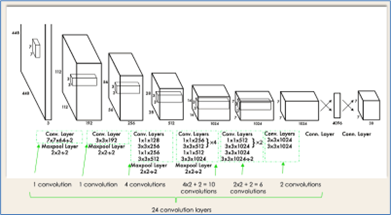
\includegraphics[width=1\columnwidth]{bab2/Gambar/Picture30.png}
	\end{center}
	\vspace{-0.2cm}
	%\rule{\columnwidth}{0.1pt}
	\captionsetup{justification=centering}
	\caption{Arsitektur YOLO dari \textit{Original Paper}\\(J. Redmon et al., 2015)}\label{img:Arsitektur-YOLO}
\end{figure}
%%%%%%%%%%%%%%%%%%%%%%%%%% GAMBAR %%%%%%%%%%%%%%%%%%%%%%%%%%%%%%

Arsitektur YOLO bekerja sebagai berikut: 
\begin{itemize}
	\item Mengubah ukuran gambar input menjadi 448x448 sebelum melalui \textit{convolutional network}. 
	
	\item Konvolusi 1x1 pertama kali diterapkan untuk mengurangi jumlah saluran, yang kemudian diikuti oleh konvolusi 3x3 untuk menghasilkan output kuboid. 
	
	\item Fungsi aktivasi ReLU, kecuali lapisan terakhir, yang menggunakan fungsi aktivasi linier.
	
	\item Beberapa Teknik tambahan, seperti normalisasi batch dan droput, masing-masing mengatur model dan mencegah overfitting. 
\end{itemize}

\subsection{Cara kerja Deteksi Objek YOLO}
\hspace{1,2cm}Berikut ini adalah proses bagaimana YOLO melakukan deteksi objek untuk mendapatkan gambar (b) dari gambar (a) pada Gambar \ref{img:Cara-Kerja-YOLO}.

%%%%%%%%%%%%%%%%%%%%%%%%%% GAMBAR %%%%%%%%%%%%%%%%%%%%%%%%%%%%%%
\begin{figure}[H]
	\vspace{-0.1cm}
	%\rule{\columnwidth}{0.1pt}
	\begin{center}
		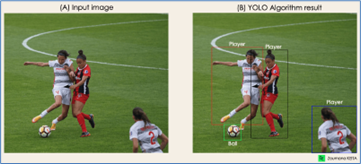
\includegraphics[width=0.9\columnwidth]{bab2/Gambar/Picture31.png}
	\end{center}
	\vspace{-0.2cm}
	%\rule{\columnwidth}{0.1pt}
	\captionsetup{justification=centering}
	\caption{(A) Input Image dan (B) Hasil Algoritma YOLO\\(Sumber: Z. Kelta, 2022)}\label{img:Cara-Kerja-YOLO}
\end{figure}
%%%%%%%%%%%%%%%%%%%%%%%%%% GAMBAR %%%%%%%%%%%%%%%%%%%%%%%%%%%%%%

Algoritma YOLO bekerja berdasarkan empat pendekatan, sebagai berikut:
\begin{enumerate}[label=(\alph*)]
	\item \textit{Residual Blocks}(Blok Sisa)
	
	Langkah pertama dimulai dengan membagi gambar asli (A) menjadi sel grid (NxN) dengan bentuk yang sama, di mana N dalam hal ini adalah 4x4 grid sel pada Gambar \ref{img:Residual-Blocks}. Setiap sel dalam grid bertanggung jawab untuk melokalkan dan memprediksi kelas objek yang dicakupnya, bersama dengan nilai probabilitas/kepercayaan.
	
	%%%%%%%%%%%%%%%%%%%%%%%%%% GAMBAR %%%%%%%%%%%%%%%%%%%%%%%%%%%%%%
	\begin{figure}[H]
		\vspace{-0.1cm}
		%\rule{\columnwidth}{0.1pt}
		\begin{center}
			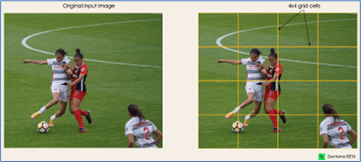
\includegraphics[width=0.9\columnwidth]{bab2/Gambar/Picture32.png}
		\end{center}
		\vspace{-0.2cm}
		%\rule{\columnwidth}{0.1pt}
		\captionsetup{justification=centering}
		\caption{Residual Blocks\\(Sumber: Z. Kelta, 2022)}\label{img:Residual-Blocks}
	\end{figure}
	%%%%%%%%%%%%%%%%%%%%%%%%%% GAMBAR %%%%%%%%%%%%%%%%%%%%%%%%%%%%%%
	
	\item \textit{Bounding Box Regression} (Regresi Kotak Pembatas)
	
	Langkah selanjutnya adalah menentukan kotak pembatas (\textit{bounding box}) yang sesuai dengan persegi Panjang yang menyoroti semua objek dalam gambar. Dapat memiliki kotak pembatas sebanyak objek di dalam gambar yang diberikan. YOLO menentukan atribut kotak pembatas ini menggunakan modul regresi tunggal dalam format berikut, dimana Y adalah representasi vector terakhir untuk setiap kotak pembatas.\\
	Y = [pc, bx, by, bh, bw, c1, c2]\\
	Ini sangat penting selama fase pelatihan model.
	\begin{itemize}
		\item pc sesuai dengan skor probabilitas dari grid yang berisi objek. Misalnya, semua grid yang berwarna merah akan memiliki skor probabilitas lebih tinggi dari nol. Gambar \ref{img:Grid-Probabilitas} adalah versi yang disederhanakan karena probabilitas setiap sel kuning adalah nol (tidak signifikan)
		
		%%%%%%%%%%%%%%%%%%%%%%%%%% GAMBAR %%%%%%%%%%%%%%%%%%%%%%%%%%%%%%
		\begin{figure}[H]
			\vspace{-0.1cm}
			%\rule{\columnwidth}{0.1pt}
			\begin{center}
				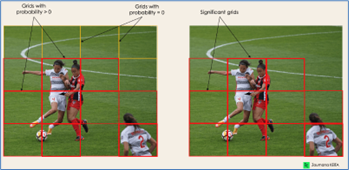
\includegraphics[width=0.9\columnwidth]{bab2/Gambar/Picture33.png}
			\end{center}
			\vspace{-0.2cm}
			%\rule{\columnwidth}{0.1pt}
			\captionsetup{justification=centering}
			\caption{Grid dengan Probabilitas\\(Sumber: Z. Kelta, 2022)}\label{img:Grid-Probabilitas}
		\end{figure}
		%%%%%%%%%%%%%%%%%%%%%%%%%% GAMBAR %%%%%%%%%%%%%%%%%%%%%%%%%%%%%%
		
		\item bx dan by adalah koordinat x dan y dari pusat kotak pembatas (\textit{center of bounding box}) sehubungan dengan grid sel pembungkus. 
		
		\item bh dan bw sesuai dengan tinggi dan lebar kotak pembatas sehubungan dengan sel grid pembungkus
		
		\item c1 dan c2 sesuai dengan dua kelas Player dan Ball, dapat memiliki kelas sebanyak yang dibutuhkan oleh pengguna.
		
		Untuk dapat memahami dan terlihat, seperti pada Gambar \ref{img:Cara-Bounding-Box} berikut.
		%%%%%%%%%%%%%%%%%%%%%%%%%% GAMBAR %%%%%%%%%%%%%%%%%%%%%%%%%%%%%%
		\begin{figure}[H]
			\vspace{-0.1cm}
			%\rule{\columnwidth}{0.1pt}
			\begin{center}
				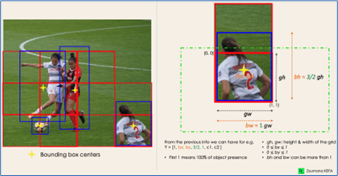
\includegraphics[width=0.9\columnwidth]{bab2/Gambar/Picture34.png}
			\end{center}
			\vspace{-0.2cm}
			%\rule{\columnwidth}{0.1pt}
			\captionsetup{justification=centering}
			\caption{Cara \textit{Bounding Box}\\(Sumber: Z. Kelta, 2022)}\label{img:Cara-Bounding-Box}
		\end{figure}
		%%%%%%%%%%%%%%%%%%%%%%%%%% GAMBAR %%%%%%%%%%%%%%%%%%%%%%%%%%%%%%
	\end{itemize}
	
	\item \textit{Intersection Over Unions} (IOU)
	
	Sebagian besar waktu, satu objek dalam gambar dapat memiliki beberapa kandidat kotak petak untuk prediksi, meskipun tidak semuanya relevan. Tujuan dari IOU (nilai antara 0 dan 1) adalah untuk membuang kotak kisi tersebut agar hanya menyimpan yang relevan. Inilah logika dari IOU:
	
	\begin{itemize}
		\item Pengguna menentukan ambang pemilihan IOU-nya, misalnya, 0,5.
		
		\item Kemudian YOLO menghitung IOU dari setiap sel grid yang merupakan area persimpangan dibagi dengan Union Area.
		
		\item Terakhir, ia mengabaikan prediksi sel kisi yang memiliki IOU $\leq$ ambang batas dan mempertimbangkannya dengan IOU > ambang batas.
	\end{itemize}
	
	Pada Gambar \ref{img:IOU} adalah ilustrasi penerapan proses pemilihan grid pada objek kiri bawah. Dapat diamati bahwa objek awalnya memiliki dua kandidat kisi, kemudian hanya "Kisi 2" yang dipilih di bagian akhir.
	
	%%%%%%%%%%%%%%%%%%%%%%%%%% GAMBAR %%%%%%%%%%%%%%%%%%%%%%%%%%%%%%
	\begin{figure}[H]
		\vspace{-0.1cm}
		%\rule{\columnwidth}{0.1pt}
		\begin{center}
			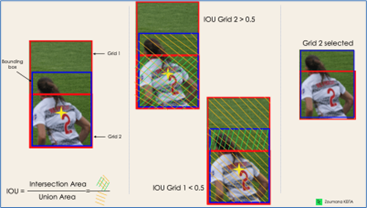
\includegraphics[width=0.9\columnwidth]{bab2/Gambar/Picture35.png}
		\end{center}
		\vspace{-0.2cm}
		%\rule{\columnwidth}{0.1pt}
		\captionsetup{justification=centering}
		\caption{IOU\\(Sumber: Z. Kelta, 2022)}\label{img:IOU}
	\end{figure}
	%%%%%%%%%%%%%%%%%%%%%%%%%% GAMBAR %%%%%%%%%%%%%%%%%%%%%%%%%%%%%%
	
	\item Non-Maximum Supression (NMS)
	
	Menetapkan ambang batas untuk IOU tidak selalu cukup karena sebuah objek dapat memiliki beberapa kotak dengan IOU di luar ambang batas, dan meninggalkan semua kotak tersebut mungkin termasuk kebisingann (\textit{noise}). Di sinilah, dapat menggunakan NMS untuk menyimpan hanya kotak dengan skor probabilitas deteksi tertinggi.
\end{enumerate}

\subsection{Perkembangan YOLO}
\hspace{1,2cm}Sejak rilis pertama YOLO pada tahun 2015, YOLO telah banyak berkembang dengan versi berbeda, seperti pada Gambar \ref{img:Perkembangan-YOLO}. 

%%%%%%%%%%%%%%%%%%%%%%%%%% GAMBAR %%%%%%%%%%%%%%%%%%%%%%%%%%%%%%
\begin{figure}[H]
	\vspace{-0.1cm}
	%\rule{\columnwidth}{0.1pt}
	\begin{center}
		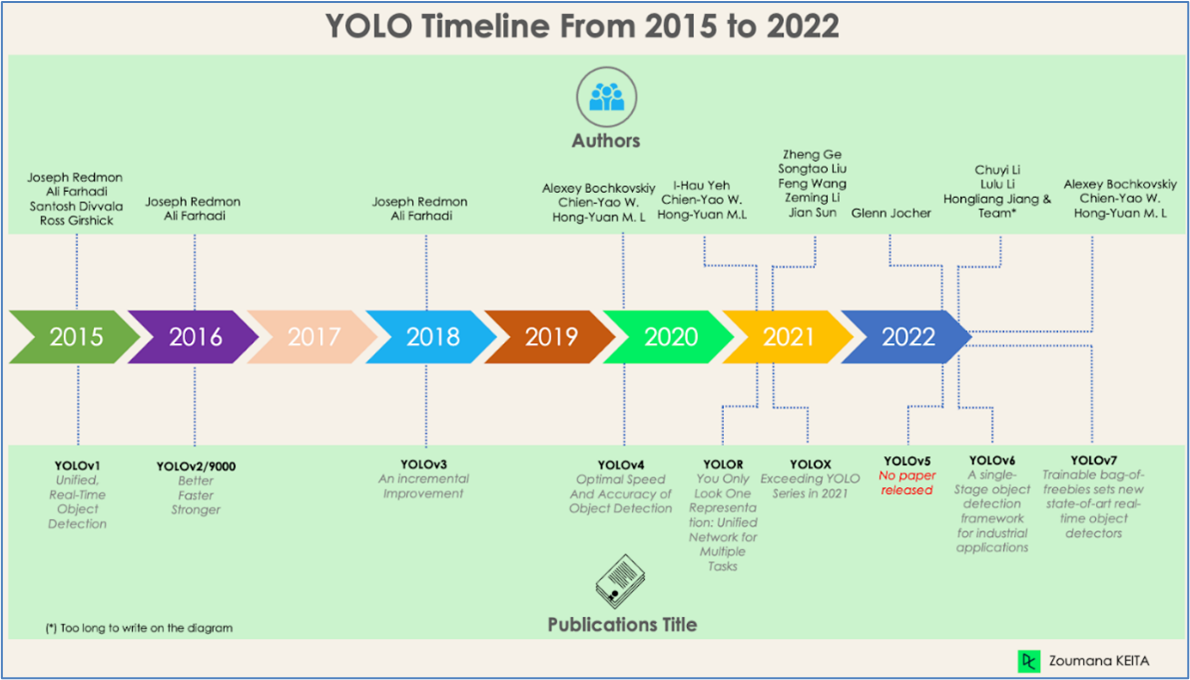
\includegraphics[width=0.9\columnwidth]{bab2/Gambar/Picture36.png}
	\end{center}
	\vspace{-0.2cm}
	%\rule{\columnwidth}{0.1pt}
	\captionsetup{justification=centering}
	\caption{Perkembangan YOLO\\(Sumber: Z. Kelta, 2022)}\label{img:Perkembangan-YOLO}
\end{figure}
%%%%%%%%%%%%%%%%%%%%%%%%%% GAMBAR %%%%%%%%%%%%%%%%%%%%%%%%%%%%%%

\begin{enumerate}
	\item YOLO atau YOLOv1
	
	Versi pertama YOLO ini adalah pengubah permainan untuk deteksi objek, karena kemampuannya mengenali objek dengan cepat dan efisien.\\
	Namun, seperti banyak solusi lainnya, versi pertama YOLO memiliki keterbatasannya sendiri:
	\begin{itemize}
		\item Kesulitan untuk mendeteksi gambar yang lebih kecil dalam sekelompok gambar, seperti sekelompok orang di stadion. Ini karena setiap kisi dalam arsitektur YOLO dirancang untuk deteksi objek tunggal.
		
		\item Kemudian, YOLO tidak berhasil mendeteksi bentuk baru atau tidak biasa.
		
		\item Terakhir, fungsi kerugian yang digunakan untuk memperkirakan kinerja pendeteksian memperlakukan kesalahan yang sama untuk kotak pembatas kecil dan besar, yang sebenarnya membuat pelokalan yang salah.
	\end{itemize}
	
	\item YOLOv2 atau YOLO9000
	
	YOLOv2 dibuat pada tahun 2016 dengan ide membuat model YOLO lebih baik, lebih cepat, dan lebih kuat.\\
	Peningkatan termasuk tetapi tidak terbatas pada penggunaan Darknet-19 sebagai arsitektur baru, normalisasi batch, resolusi input yang lebih tinggi, lapisan konvolusi dengan anchors, pengelompokan dimensi, dan (5) fitur-fitur halus.
	
	\begin{itemize}
		\item \textit{Batch Normalization}
		
		Menambahkan lapisan normalisasi batch meningkatkan kinerja sebesar 2\% mAP. Normalisasi batch ini menyertakan efek regularisasi, mencegah overfitting.
		
		\item \textit{Higher input resolution}
		
		YOLOv2 secara langsung menggunakan input 448x448 beresolusi lebih tinggi daripada 224x224, yang membuat model menyesuaikan filternya untuk bekerja lebih baik pada gambar beresolusi lebih tinggi. Pendekatan ini meningkatkan akurasi sebesar 4\% mAP, setelah dilatih selama 10 epochs pada data ImageNet.
	\end{itemize}
	
	\item YOLOv3 - Peningkatan Bertahap
	
	Perubahan tersebut terutama mencakup arsitektur jaringan baru: Darknet-53. Ini adalah jaringan saraf 106, dengan jaringan upsampling dan blok residual. Jauh lebih besar, lebih cepat, dan lebih akurat dibandingkan dengan Darknet-19, yang merupakan tulang punggung YOLOv2. Arsitektur baru ini telah bermanfaat di banyak tingkatan:
	
	\begin{itemize}
		\item Prediksi \textit{Bounding Box} Lebih Baik
		
		Model regresi logistic digunakan oleh YOLOv3 untuk memprediksi skor objektivitas untuk setiap kotak pembatas (bounding box).
		
		\item Prediksi Kelas yang Lebih Akurat
		
		Menggantikan penggunaan softmax seperti yang dilakukan di YOLOv2, pengklasifikasi logistik independen telah diperkenalkan untuk memprediksi kelas kotak pembatas secara akurat. Ini bahkan berguna saat menghadapi domain yang lebih kompleks dengan label yang tumpang tindih (Misalnya, $\rightarrow$ Pemain Sepak Bola). Menggunakan softmax akan membatasi setiap kotak hanya memiliki satu kelas, yang tidak selalu benar.
		
	\end{itemize}
	
	\item YOLOv4 - \textit{Optimal Speed dan Accuracy of Object Detection}
	
	Versi YOLO ini memiliki Kecepatan dan Akurasi Deteksi Objek Optimal dibandingkan dengan semua versi sebelumnya dan detektor objek canggih lainnya.\\
	Gambar \ref{img:KomprasiYoloV4-YoloV3} menunjukkan YOLOv4 mengungguli YOLOv3 dan FPS dalam kecepatan masing-masing sebesar 10\% dan 12\%.
	
	%%%%%%%%%%%%%%%%%%%%%%%%%% GAMBAR %%%%%%%%%%%%%%%%%%%%%%%%%%%%%%
	\begin{figure}[H]
		\vspace{-0.1cm}
		%\rule{\columnwidth}{0.1pt}
		\begin{center}
			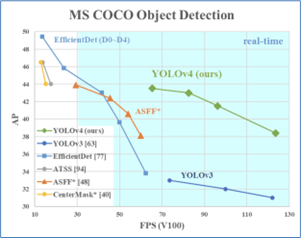
\includegraphics[width=0.8\columnwidth]{bab2/Gambar/Picture37.png}
		\end{center}
		\vspace{-0.2cm}
		%\rule{\columnwidth}{0.1pt}
		\captionsetup{justification=centering}
		\caption{Komparasi YOLOv4 dengan YOLOv3 dan \textit{state-of-the-art} Deteksi Objek Lain \\(Sumber: Z. Kelta, 2022)}\label{img:KomprasiYoloV4-YoloV3}
	\end{figure}
	%%%%%%%%%%%%%%%%%%%%%%%%%% GAMBAR %%%%%%%%%%%%%%%%%%%%%%%%%%%%%%
	YOLOv4 dirancang khusus untuk sistem produksi dan dioptimalkan untuk komputasi paralel.\\
	\textit{Backbone} arsitektur YOLOv4 adalah CSPDarknet53, jaringan yang berisi 29 lapisan konvolusi dengan filter 3 x 3 dan sekitar 27,6 juta parameter.\\
	Arsitektur ini, dibandingkan dengan YOLOv3, menambahkan informasi berikut untuk deteksi objek yang lebih baik:
	
	\begin{itemize}
		\item \textit{Spatial Pyramid Pooling} (SPP) secara signifikan meningkatkan bidang reseptif, memisahkan fitur konteks yang paling relevan, dan tidak memengaruhi kecepatan jaringan.
		
		\item Menggantikan \textit{Feature Pyramid Network} (FPN) yang digunakan di YOLOv3, YOLOv4 menggunakan PANet untuk agregasi parameter dari tingkat deteksi yang berbeda.
		
		\item Augmentasi data menggunakan teknik mosaik yang menggabungkan empat gambar pelatihan selain pendekatan pelatihan permusuhan diri.
		
		\item Menggunakan pemilihan hyper-parameter yang optimal menggunakan algoritma genetika.
		
	\end{itemize}
	
	\item YOLOR - You Only Look One Representation
	
	Sebagai \textit{Unified Network for Multiple Tasks}, YOLOR didasarkan pada jaringan terpadu yang merupakan kombinasi dari pendekatan pengetahuan eksplisit dan implisit.
	
	%%%%%%%%%%%%%%%%%%%%%%%%%% GAMBAR %%%%%%%%%%%%%%%%%%%%%%%%%%%%%%
	\begin{figure}[H]
		\vspace{-0.1cm}
		%\rule{\columnwidth}{0.1pt}
		\begin{center}
			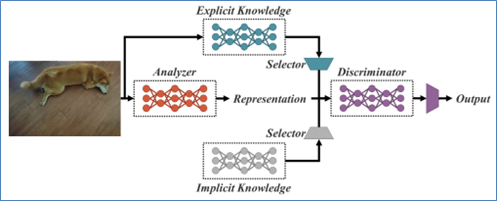
\includegraphics[width=0.8\columnwidth]{bab2/Gambar/Picture38.png}
		\end{center}
		\vspace{-0.2cm}
		%\rule{\columnwidth}{0.1pt}
		\captionsetup{justification=centering}
		\caption{Unified Network Architecture\\(Sumber: C. Y. Wang et al, 2021}\label{img:Unified-Network-Architecture}
	\end{figure}
	%%%%%%%%%%%%%%%%%%%%%%%%%% GAMBAR %%%%%%%%%%%%%%%%%%%%%%%%%%%%%%
		Pengetahuan eksplisit adalah pembelajaran normal atau conscious learning. Pembelajaran implisit di sisi lain dilakukan secara tidak sadar (dari pengalaman).\\
		Menggabungkan kedua teknik ini, YOLOR mampu menciptakan arsitektur yang lebih kuat berdasarkan tiga proses: (1) penyelarasan fitur, (2) penyelarasan prediksi untuk deteksi objek, dan (3) representasi kanonis untuk pembelajaran multi-tugas.\\
		Salah satu yang mengalami peningkatan adalah penjajaran prediksi. Pendekatan ini memperkenalkan representasi implisit ke dalam peta fitur dari setiap jaringan piramida fitur (FPN), yang meningkatkan presisi sekitar 0,5\%.\\
		Dari grafik berikut, dapat diamati bahwa YOLOR mencapai kecepatan inferensi data MS COCO yang canggih dibandingkan dengan model lain seperti pada Gambar \ref{img:Performance-YOLOR-YOLOV4}.
		
	%%%%%%%%%%%%%%%%%%%%%%%%%% GAMBAR %%%%%%%%%%%%%%%%%%%%%%%%%%%%%%
	\begin{figure}[H]
		\vspace{-0.1cm}
		%\rule{\columnwidth}{0.1pt}
		\begin{center}
			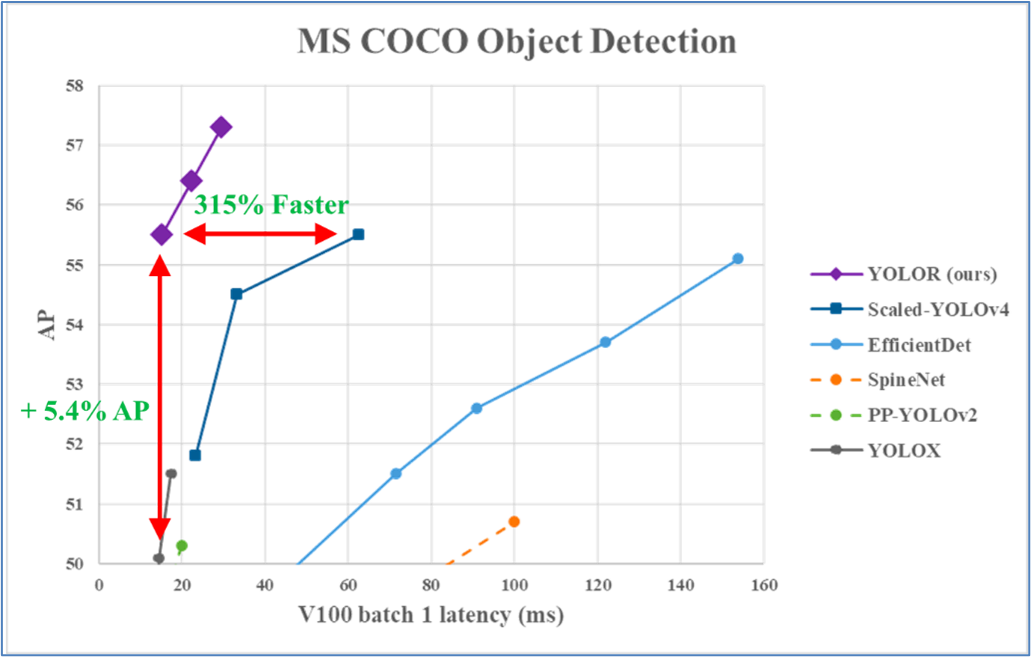
\includegraphics[width=0.8\columnwidth]{bab2/Gambar/Picture39.png}
		\end{center}
		\vspace{-0.2cm}
		%\rule{\columnwidth}{0.1pt}
		\captionsetup{justification=centering}
		\caption{Performance YOLOR vs YOLOv4 dan Model Lainnya\\(Sumber: C. Y. Wang et al, 2021}\label{img:Performance-YOLOR-YOLOV4}
	\end{figure}
	%%%%%%%%%%%%%%%%%%%%%%%%%% GAMBAR %%%%%%%%%%%%%%%%%%%%%%%%%%%%%%
	
	\item YOLOX - Exciding \textit{YOLO Series in 2021}
	
	Ini menggunakan baseline yang merupakan versi modifikasi dari YOLOv3, dengan Darknet-53 sebagai \textit{backbone}.\\
	Diterbitkan dalam makalah \textit{Exceeding} YOLO \textit{Series in 2021}, YOLOX menghadirkan empat karakteristik utama berikut untuk membuat model yang lebih baik dibandingkan dengan versi yang lebih lama.
	
	\begin{itemize}
		\item Kepala terpisah yang efisien: Coupled head yang digunakan pada versi YOLO sebelumnya terbukti mengurangi performa model. YOLOX menggunakan decoupled sebagai gantinya, yang memungkinkan pemisahan tugas klasifikasi dan lokalisasi, sehingga meningkatkan kinerja model.
		
		\item Augmentasi data yang kuat: Integrasi Mosaic dan MixUp ke dalam pendekatan augmentasi data sangat meningkatkan kinerja YOLOX.
		
		\item \textit{Anchor free system}: Algoritma \textit{anchor-based} melakukan pengelompokan di bawah tenda, yang meningkatkan waktu inferensi. Menghapus mekanisme jangkar di YOLOX mengurangi jumlah prediksi per gambar, dan meningkatkan waktu inferensi secara signifikan.
		
		\item SimOTA untuk penetapan label: Pergantian penggunaan pendekatan interseksi penyatuan (IoU), penulis memperkenalkan SimOTA, strategi penetapan label yang lebih kuat yang mencapai hasil canggih dengan tidak hanya mengurangi waktu pelatihan tetapi juga menghindari masalah hiperparameter tambahan. Selain itu, ini meningkatkan peta deteksi sebesar 3\%.
		
	\end{itemize}
	
	\item YOLOv5
	
	YOLOv5, dibandingkan dengan versi lain, tidak memiliki makalah penelitian yang diterbitkan, dan ini adalah versi YOLO pertama yang diimplementasikan di Pytorch, bukan di Darknet.\\
	Dirilis oleh Glenn Jocher pada Juni 2020, YOLOv5, mirip dengan YOLOv4, menggunakan CSPDarknet53 sebagai tulang punggung arsitekturnya. Rilis ini mencakup lima ukuran model yang berbeda: YOLOv5s (terkecil), YOLOv5m, YOLOv5l, dan YOLOv5x (terbesar).\\
	Salah satu peningkatan besar dalam arsitektur YOLOv5 adalah integrasi lapisan Fokus, yang diwakili oleh satu lapisan, yang dibuat dengan mengganti tiga lapisan pertama YOLOv3. Integrasi ini mengurangi jumlah lapisan, dan jumlah parameter dan juga meningkatkan kecepatan maju dan mundur tanpa dampak besar pada peta.\\
	Ilustrasi Gambar \ref{img:Perbandingan-YOLOv4-YOLOv5} membandingkan waktu pelatihan antara YOLOv4 dan YOLOv5.
	
	%%%%%%%%%%%%%%%%%%%%%%%%%% GAMBAR %%%%%%%%%%%%%%%%%%%%%%%%%%%%%%
	\begin{figure}[H]
		\vspace{-0.1cm}
		%\rule{\columnwidth}{0.1pt}
		\begin{center}
			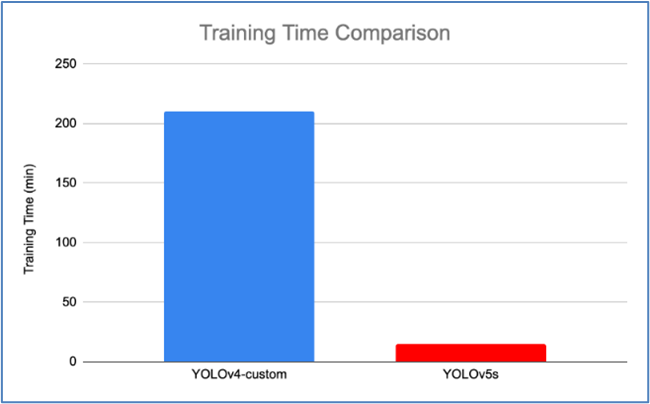
\includegraphics[width=0.6\columnwidth]{bab2/Gambar/Picture40.png}
		\end{center}
		\vspace{-0.2cm}
		%\rule{\columnwidth}{0.1pt}
		\captionsetup{justification=centering}
		\caption{Perbandingan Waktu Pelatihan antara YOLOv4 dan YOLOv5\\(Sumber: J. Nelson, 2020}\label{img:Perbandingan-YOLOv4-YOLOv5}
	\end{figure}
	%%%%%%%%%%%%%%%%%%%%%%%%%% GAMBAR %%%%%%%%%%%%%%%%%%%%%%%%%%%%%%
	
	\item YOLOv6
	
	Didedikasikan untuk aplikasi industri dengan desain efisien yang ramah perangkat keras dan kinerja tinggi, kerangka kerja YOLOv6 (MT-YOLOv6) dirilis oleh Meituan, sebuah perusahaan e-commerce Tiongkok.\\
	Ditulis dalam Pytorch, versi baru ini bukan bagian dari YOLO resmi tetapi tetap diberi nama YOLOv6 karena tulang punggungnya terinspirasi oleh arsitektur YOLO satu tahap yang asli.\\
	YOLOv6 memperkenalkan tiga peningkatan signifikan pada YOLOv5 sebelumnya: desain tulang punggung dan leher yang ramah perangkat keras, kepala terpisah yang efisien, dan strategi pelatihan yang lebih efektif.\\
	YOLOv6 memberikan hasil yang luar biasa dibandingkan dengan versi YOLO sebelumnya dalam hal akurasi dan kecepatan pada dataset COCO seperti yang diilustrasikan pada Gambar \ref{img:Performance-YOLOv6}
	
	%%%%%%%%%%%%%%%%%%%%%%%%%% GAMBAR %%%%%%%%%%%%%%%%%%%%%%%%%%%%%%
	\begin{figure}[H]
		\vspace{-0.1cm}
		%\rule{\columnwidth}{0.1pt}
		\begin{center}
			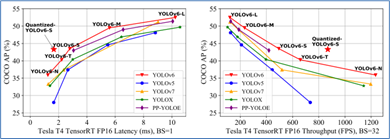
\includegraphics[width=1\columnwidth]{bab2/Gambar/Picture41.png}
		\end{center}
		\vspace{-0.2cm}
		%\rule{\columnwidth}{0.1pt}
		\captionsetup{justification=centering}
		\caption{Comparison of state-of-the-art efficient object detectors. All models are tested with TensorRT 7 except that the quantized model is with TensorRT 8\\(Sumber: C. Li et al, 2022}\label{img:Performance-YOLOv6}
	\end{figure}
	%%%%%%%%%%%%%%%%%%%%%%%%%% GAMBAR %%%%%%%%%%%%%%%%%%%%%%%%%%%%%%
	
	\begin{itemize}
		\item YOLOv6-N mencapai 35,9\% AP pada dataset COCO dengan throughput 1234 (throughput) FPS pada GPU NVIDIA Tesla T4.
		
		\item YOLOv6-S mencapai AP 43,3\% yang canggih pada 869 FPS.
		
		\item YOLOv6-M dan YOLOv6-L juga mencapai kinerja akurasi yang lebih baik masing-masing sebesar 49,5\% dan 52,3\% dengan kecepatan inferensi yang sama.
		
	\end{itemize}
	
	\item YOLOv7
	
	YOLOv7 dirilis pada Juli 2022 di Paper \textit{Trained bag-of-freebies set state-of-the-art real-time object detector}. Versi ini membuat langkah signifikan di bidang deteksi objek, dan melampaui semua model sebelumnya dalam hal akurasi dan kecepatan.
	
	%%%%%%%%%%%%%%%%%%%%%%%%%% GAMBAR %%%%%%%%%%%%%%%%%%%%%%%%%%%%%%
	\begin{figure}[H]
		\vspace{-0.1cm}
		%\rule{\columnwidth}{0.1pt}
		\begin{center}
			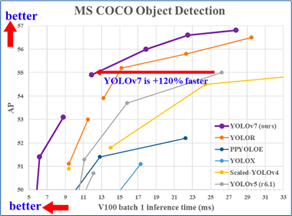
\includegraphics[width=1\columnwidth]{bab2/Gambar/Picture42.png}
		\end{center}
		\vspace{-0.2cm}
		%\rule{\columnwidth}{0.1pt}
		\captionsetup{justification=centering}
		\caption{Perbandingan YOLOv7 inference time dengan real-time object detector lainnya\\(Sumber: C. Y. Wang et al, 2022}\label{img:Performance-YOLOv7}
	\end{figure}
	%%%%%%%%%%%%%%%%%%%%%%%%%% GAMBAR %%%%%%%%%%%%%%%%%%%%%%%%%%%%%%
	YOLOv7 telah membuat perubahan besar dalam (1) arsitekturnya dan (2) pada tingkat bag-of-freebies yang dapat dilatih:
	
	\begin{itemize}
		\item Level Aristektur
		
		YOLOv7 mereformasi arsitekturnya dengan mengintegrasikan Extended Efficient Layer Aggregation Network (E-ELAN) yang memungkinkan model mempelajari fitur yang lebih beragam untuk pembelajaran yang lebih baik.\\
		Selain itu, YOLOv7 menskalakan arsitekturnya dengan menggabungkan arsitektur model asalnya seperti YOLOv4, Scaled YOLOv4, dan YOLO-R. Hal ini memungkinkan model untuk memenuhi kebutuhan kecepatan inferensi yang berbeda.
		
		%%%%%%%%%%%%%%%%%%%%%%%%%% GAMBAR %%%%%%%%%%%%%%%%%%%%%%%%%%%%%%
		\begin{figure}[H]
			\vspace{-0.1cm}
			%\rule{\columnwidth}{0.1pt}
			\begin{center}
				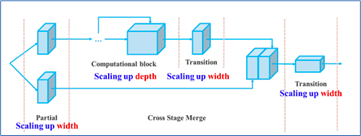
\includegraphics[width=1\columnwidth]{bab2/Gambar/Picture43.png}
			\end{center}
			\vspace{-0.2cm}
			%\rule{\columnwidth}{0.1pt}
			\captionsetup{justification=centering}
			\caption{\textit{Compound scaling up depth and width for concatenation-based model}\\(Sumber: C. Y. Wang et al, 2022}\label{img:Compund-Scaling}
		\end{figure}
		%%%%%%%%%%%%%%%%%%%%%%%%%% GAMBAR %%%%%%%%%%%%%%%%%%%%%%%%%%%%%%
		
		\item Trainable bag-of-freebies
		
		Istilah bag-of-freebies mengacu pada peningkatan akurasi model tanpa meningkatkan biaya pelatihan, dan inilah alasan mengapa YOLOv7 tidak hanya meningkatkan kecepatan inferensi tetapi juga akurasi deteksi.
		
	\end{itemize}
\end{enumerate}

\section{Object Based Image Analysis (OBIA)}
\hspace{1,2cm}OBIA merupakan teknik klasifikasi yang tidak hanya memandang rona dan tekstur piksel namun berdasarkan dari kesatuan objek, atau dapat dikatakan OBIA adalah pendekatan yang proses klasifikasinya tidak hanya mempertimbangkan aspek spectral naum aspek spasial objek. Data citra penginderaan jauh yang digunakan untuk klasifikasi ini biasanya menggunakan data citra penginderaan jauh resolusi tinggi seperti QUickbird, Ikonos, World View, dll. Klasifikasi ini hamper mirip dengan klasifikasi unsupervised, akan tetapi basis dari klasifikasi OBIA yaitu dengan segmentasi \citep{OBIA}.

OBIA mengelompokkan gambar yang mengelompokkan piksel kecil menjadi objek vektor. Alih-alih berbasis per-pixel, segmentasi secara otomatis mendigitalkan gambar untuk pengguna (GIS Geography, 2020).

%%%%%%%%%%%%%%%%%%%%%%%%%% GAMBAR %%%%%%%%%%%%%%%%%%%%%%%%%%%%%%
\begin{figure}[H]
	\vspace{-0.1cm}
	%\rule{\columnwidth}{0.1pt}
	\begin{center}
		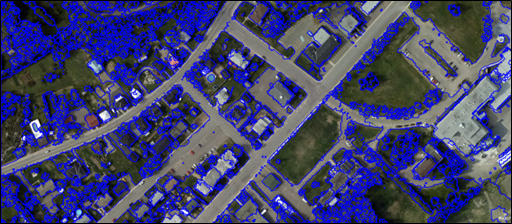
\includegraphics[width=1\columnwidth]{bab2/Gambar/Picture44.png}
	\end{center}
	\vspace{-0.2cm}
	%\rule{\columnwidth}{0.1pt}
	\captionsetup{justification=centering}
	\caption{OBIA Segmentasi Proses Pengelompokkkan Pixel yang hampir sama ke dalam Objek\\(Sumber: GISGeography, 2020)}\label{img:OBIA-Segmentasi-Proses}
\end{figure}
%%%%%%%%%%%%%%%%%%%%%%%%%% GAMBAR %%%%%%%%%%%%%%%%%%%%%%%%%%%%%%

Apa yang dilakukan segmentasi adalah meniru apa yang dilakukan mata pengguna. Tetapi dengan objek tersegmentasi ini, pengguna menggunakan properti spektral, geometris, dan spasialnya untuk mengklasifikasikan ke dalam tutupan lahan.

%%%%%%%%%%%%%%%%%%%%%%%%%% GAMBAR %%%%%%%%%%%%%%%%%%%%%%%%%%%%%%
\begin{figure}[H]
	\vspace{-0.1cm}
	%\rule{\columnwidth}{0.1pt}
	\begin{center}
		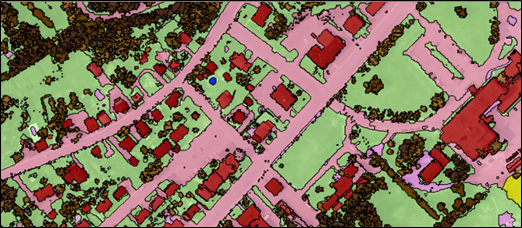
\includegraphics[width=1\columnwidth]{bab2/Gambar/Picture45.png}
	\end{center}
	\vspace{-0.2cm}
	%\rule{\columnwidth}{0.1pt}
	\captionsetup{justification=centering}
	\caption{OBIA Klasifikasi menggunakan shape, size, dan spectral properties objek untuk klasifikasi setiap objek}\label{img:OBIA-Klasifikasi}
\end{figure}
%%%%%%%%%%%%%%%%%%%%%%%%%% GAMBAR %%%%%%%%%%%%%%%%%%%%%%%%%%%%%%

Dua prinsip dasar OBIA adalah klasifikasi dan segmentasi. Segmentasi adalah memecah gambar menjadi objek yang mewakili fitur berbasis darat, sedangkan Klasifikasi adalah mengklasifikasi objek-objek tersebut menggunakan bentuk, ukuran, sifat spasial dan spektralnya. Analis sering menggunakan statistik ini untuk mengklasifikasikan tutupan lahan menggunakan OBIA, yaitu \textit{trees} (pohon) memiliki ketinggian yang bervariasi (standar deviasi \textit{normalized Digital Surface Model} (nDSM)) yang merupakan model elevasi yang menangkap fitur alami dan fitur buatan, seperti gedung, pohon, kabel listrik, dan objek lainnya. Di samping itu, memiliki reflektansi inframerah-dekat yang tinggi (\textit{normalized difference vegetation index} (NDVI) tinggi), sedangkan \textit{grass} memiliki pendek (nDSM rendah), datar (deviasi standar nDSM rendah) dan memiliki reflektansi inframerah-dekat sedang (NDVI sedang). NDVI digunakan untuk mengukur indeks yang menggambarkan tingkat kepadatan, kehijauan suatu tanaman dan kondisi dari suatu vegetasi.

\section{Sentinel-2}
\hspace{1,2cm}Data yang digunakan dalam penelitian ini diambil dari gambar citra satelit Sentinel-2. Sentinel-2 diluncurkan sebagai bagian dari program Copernicus Komisi Eropa pada tanggal 23 Juni 2015 yang dirancang khusus untuk memberikan banyak data dan citra. Satelit dilengkapi dengan sensor multispectral opto-elektronik untuk survei dengan resoulsi Sentinel-2 yaitu 10 hingga 60m di zona spekatral tampak, VNIR, SWIR, termasuk 13 saluran spectral yang memastikan penangkapan perbedaan dalam keadaan vegetasi, termasuk perubahan temporal, dna juga meminimalkan dampkan kualitas fotografi atmosfer. Sentinel-2 memiliki dua satelit dalam misi memungkinkan survei berulang setiap 5 hari di ekuator dan 2-3 hari di garis lintang tengah (EOS, 2020). 

Misi Sentinel-2 terdiri dari dua satelit yang dikembangkan untuk mendukung vegetasi, tutupan lahan, dan pemantauan lingkungan. Satelit Sentinel-2A diluncurkan oleh European Space Agency (ESA) pada 23 Juni 2015, dan beroperasi di orbit sinkron matahari dengan siklus berulang 10 hari. Setelit kedua yaitu Sentinel-2B diluncurkan pada 7 Maret 2017 dan beroperasi dengan akuisisi data yang tersedia di EarthExplorer (USGS EROS, 2020). 

Terdapat Perbandingan antara Sentinel-2 dengan UAV Drone, seperti pada Tabel 2.2.

%%% BENERIN TABEL

\section{Pertanian Presisi}
\hspace{1,2cm}Pertanian presisi atau precision agriculture merupakan suatu sistem pertanian yang mengintegrasikan penggunaan teknologi dalam mengumpulkan informasi, sehingga dapat melakukan proses pertanian secara presisi atau dengan input, tempat, dan waktu yang tepat. Istilah presisi berarti akurat, terakar, dan terukur. Pertanian presisi disebut juga menggunakan input pertanian yang tepat dengan teknik, jumlah, tempat, dan waktu yang tepat untuk menghasilkan produksi panen secara maksimal. Input pertanian meliputi seperti pemupukan, herbisida, insektisida, benih, dan lainnya. Meskipun untuk melakukan pertanian secara akurat ini membutuhkan banyak informasi, cenderung kompleks untuk kebanyakan petani, dan membutuhkan kerjasama dari berbagai multidisiplin ilmu, namun sistem pertanian presisi mampu meingkatkan laba, mengurangi limbah, mengurangi biaya produksi, dan menjaga kualitas lingkungan (J. Taylor et al., 2016). 

Pertanian presisi (PA) merupakan ilmu untuk meningkatkan hasil panen dan membantu keputusan manajemen menggunakan sensor dan alat analisis teknologi tinggi. Pertanian presisi adalah konsep yang digunakan untuk meningkatkan produksi, mengurangi waktu kerja, dan memastikan pengelolaan seperti pupuk, irigasi, dan lainnya berjalan efektif. Perkembangan teknologi, khususnya ketersediaan citra satelit beresolusi tinggi, perkembangan teknologi kendaraan udara tak berawak (UAV), menunjukkan bahwa adopsi sumber data penginderaan jauh dalam pertanian presisi mengalami peningkatan (P. Singh et al., 2020). 

Siklus pertanian presisi terdiri dari tahapan seperti Gambar 2.46.
%%%%%%%%%%%%%%%%%%%%%%%%%% GAMBAR %%%%%%%%%%%%%%%%%%%%%%%%%%%%%%
\begin{figure}[H]
	\vspace{-0.1cm}
	%\rule{\columnwidth}{0.1pt}
	\begin{center}
		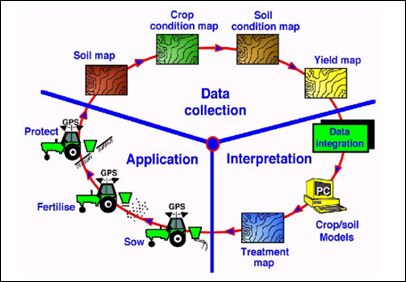
\includegraphics[width=1\columnwidth]{bab2/Gambar/Picture46.png}
	\end{center}
	\vspace{-0.2cm}
	%\rule{\columnwidth}{0.1pt}
	\captionsetup{justification=centering}
	\caption{Siklus Pertanian Presisi\\(Sumber: A. Comparetti, 2011)}\label{img:Siklus-Pertanian-Presisi}
\end{figure}
%%%%%%%%%%%%%%%%%%%%%%%%%% GAMBAR %%%%%%%%%%%%%%%%%%%%%%%%%%%%%%
\begin{itemize}
	\item Pengukuran parameter tanah dan tanaman dengan bantuan pemetaan spasial dan pemantauan kondisi cuaca setempat (pengumpulan data);
	
	\item pemetaan parameter tanah dan tanaman dalam lapangan (pengumpulan data);
	
	\item pemetaan dan integrasi data dengan bantuan aplikasi (interpretasi);
	
	\item pemantauan kesuburan dan penaburan (aplikasi);
	
\end{itemize}
Dalam menerapkan pertanian presisi diperlukan instrumen berikut (A. Comparetti, 2011):

\begin{itemize}
	\item Sistem penentuan posisi satelit, untuk penginderaan posisi di mana setiap parameter lapangan yang diukur harus direferensikan secara geografis dan, kemudian, juga posisi di mana input (seperti, tanaman, lahan) yang terdeteksi oleh  mesin dapat diterapkan kebutuhannya di setiap area lahan (zona pengelolaan).
	
	\item Sensor, untuk mengukur parameter tanah dan tanaman di lapangan.
	
	\item Perangkat (devices), untuk menyiapkan dan mengontrol aplikasi input tanaman tingkat variabel spasial.
	
	\item Perangkat lunak, untuk membuat peta parameter tanah dan tanaman dalam lahan dan aplikasi input tanaman dengan data dari citra penginderaan, dan juga untuk menginterpretasikan data terukur;
	
\end{itemize}

\section{Kelapa Sawit}
\hspace{1,2cm}Kelapa sawit adalah tanaman sejenis palma berakar serabut atau monokotil. Bagian tanaman yang bernilai ekonomis adalah buah. Masing-masing dari seribu atau lebih buah dalam tandan buah segar itu terdiri dari inti sawit (kernel) yang dikelilingi) oleh daging buah (mesocarp). Di pabrik kelapa sawit, sangat sedikit buah yang terbuang sia-sia karena pabrik tersebut mengubah setiap buah kelapa sawit menjadi minyak kelapa sawit dan minyak inti sawit), bahkan limbah dari setiap buah sawitpun di daur ulang di perkebunan sebagai pupuk atau diolah sebagai bahan bakar biomass. Sangat sedikit sekali buah kelapa sawit terbuang karena baik inti kelapa sawit dan dagingnya sama-sama digunakan untuk menghasilkan minyak.

%%%%%%%%%%%%%%%%%%%%%%%%%% GAMBAR %%%%%%%%%%%%%%%%%%%%%%%%%%%%%%
\begin{figure}[H]
	\vspace{-0.1cm}
	%\rule{\columnwidth}{0.1pt}
	\begin{center}
		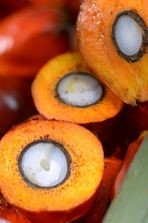
\includegraphics[width=0.3\columnwidth]{bab2/Gambar/Picture47.jpg}
	\end{center}
	\vspace{-0.2cm}
	%\rule{\columnwidth}{0.1pt}
	\captionsetup{justification=centering}
	\caption{Buah Kelapa Sawit(Inti dan Daging Sawit)}\label{img:Buah-Kelapa-Sawit}
\end{figure}
%%%%%%%%%%%%%%%%%%%%%%%%%% GAMBAR %%%%%%%%%%%%%%%%%%%%%%%%%%%%%%

Satu tandan tanaman dewasa beratnya mencapai 20 - 35 kg, bahkan ada yang mencapai di atas 40 kg, tergantung pada perawatan. Tandan tersusun dari 200 - 600 buah masing-masing sekitar 20-35 gram. Buah diambil minyaknya dengan hasil sabut (daging buah/mesocarp) menghasilkan minyak kasar (CPO) 20-26\%, inti sawit sebanyak 6\% yang menghasilkan minyak inti (PKO) 3-4\%. Kadar \% dihitung dari berat tandan buah segar (Smart Agribusiness and Food, 2017).

\begin{enumerate}[label=(\alph*)]
	\item Usia Tanam
	
	Umur atau usia ekonomis tanaman kelapa sawit yang dibudidayakan bisa mencapai usia hingga 25 tahun. Pada usia tanam sudah tinggi, sehingga sulit dipanen, tandanya sudah jarang sehingga secara perhitungan tidak ekonomis lagi. Pengelompokkan berdasarkan masa berbuah (PTPN, 2018), seperti Tabel \ref{tbl:Pengelompokkan-Berdasarkan-Masa-Berubah} berikut ini:
	
	%%%%%%%%%%%%%%%%%%%%%%%TABEL SEDERHANA%%%%%%%%%%%%%%%%%%%%%%%%%
	\begin{singlespace}
		\begin{table}[H]
			\centering
			\caption{Pengelompokkan Berdasarkan Masa Berbuah}
			\label{tbl:Pengelompokkan-Berdasarkan-Masa-Berubah}
			\begin{tabular}{|p{6cm}|p{6cm}|}
				\hline
				\multicolumn{1}{|c|}{Kelompok}   & Masa Berbuah (Tahun) \\ \hline
				Tanaman Belum Menghasilkan (TBM) & 0-3                  \\ \hline
				Tanaman Menghasilkan             & \textgreater{}3      \\ \hline
			\end{tabular}
		\end{table}
	\end{singlespace}
	%%%%%%%%%%%%%%%%%%%%%%%TABEL SEDERHANA%%%%%%%%%%%%%%%%%%%%%%%%%
	
	\item Produktivitas Tanaman Kelapa Sawit Menurut Umur Tanaman
	
	Produktivitas tanaman kelapa sawit (tandan buah segar (TBS)) menurut umur tanaman dalam Kondisi Kebun Percobaan Balit Marihat berdasarkan PTPN. VII tahun 1993 dalam \textit{lecture note} "Budi Daya Kelapa Sawit" (S. Yahya \& Suwarto, 2021), seperti Tabel 2.4. berikut ini:
	
	%%%%%%%%%%%%%%%%%%%%%%%TABEL SEDERHANA%%%%%%%%%%%%%%%%%%%%%%%%%
	\begin{singlespace}
		\begin{table}[H]
			\centering
			\caption{Produktivitas Tanaman Kelapa Sawit Menurut Umur Tanaman dalam Kondisi Kebun Percobaan Balit Marihat}
			\label{tbl:Produktivitas-Tanaman-Kelapa-Sawit}
			\begin{tabular}{|c|c|}
			\hline
			
			Umur Di Lapangan (Tahun) & \begin{tabular}[c]{@{}c@{}}Produksi    Produksi TBS\\ (ton/ha/Thn)\end{tabular} \\ \hline
			
			4 & 8 \\ \hline
			
			5 & 15 \\ \hline
			
			6 & 17 \\ \hline
			
			7 & 18 \\ \hline
			
			8 & 20 \\ \hline
			
			9 & 21 \\ \hline
			
			10 & 23 \\ \hline
			
			11 & 25 \\ \hline
			
			12 & 26 \\ \hline
			
			13 & 30 \\ \hline
			
			14 & 30 \\ \hline
			
			15 & 30 \\ \hline
			
			16 & 30 \\ \hline
			
			17 & 29 \\ \hline
			
			18 & 28 \\ \hline
			
			19 & 28 \\ \hline
			
			20 & 25 \\ \hline
			
			21 & 23 \\ \hline
			
			22 & 20 \\ \hline
			
			23 & 18 \\ \hline
			
			24 & 18 \\ \hline
			
			25 & 18 \\ \hline
				
				
			\end{tabular}
		\end{table}
	\end{singlespace}
	%%%%%%%%%%%%%%%%%%%%%%%TABEL SEDERHANA%%%%%%%%%%%%%%%%%%%%%%%%%
	
	\item Jarak Tanam Pohon Kelapa Sawit
	
	Penanaman kelapa sawit yang baik di lapangan akan menghasilkan tanaman yang sehat (tidak ada yang abnormal, non produktif, mati) dan seraam, sehingga tanaman akan cepat berproduksi (kurang dari 30 bulan setelah tanam) dengan hasil awal yang tinggi. Penanaman kelapa sawit perlu diatur dengan jarak tanam yang sesuai. Jumlah populasi tanaman persatuan luas ditentukan oleh beberapa faktor yaitu jarak tanam yang digunakan dan model jarak tanam yang digunakan. Misalnya, pada penanaman kelapa sawit dengan jarak tanam 9 m x 9 m, akan memiliki jumlah populasi tanaman yang berbeda bila model jarak tanam yang digunakan berbeda (segitiga atau segiempat) (S. Nora \& C D. Mual, 2018). 
	
	\begin{enumerate}[label=(\alph*)]
		\item Penentuan jarak tanam di lapangan harus disesuaikan dengan karakter tanaman, tingkat kesuburan, topografi, dan kondisi setempat; 
		
		\item Jarak yang teratur hanya dapat dicapai bila dilakukan pemancangan yang baik; 
		
		\item Sistem jarak tanam pada kelapa sawit berkaitan erat dengan populasi per ha (kerapatan pohon/ha) dan produksi tandan setiap pohon; 
		
		\item Kerapatan tanaman (jumlah pohon/ha) yang lebih banyak akan mempengaruhi ruang tumbuh tanaman. 
		Terdapat 2 cara dalam menghitung jarak tanam kelapa sawit, yaitu bujur sangkar dan segitiga. 
		
		\begin{enumerate}
			\item Perhitungan Bujur Sangkar
			
			Perhitungannya sama dengan tanaman yang mempunyai sistem pertanaman segiempat seperti Gambar \ref{img:Pola-Jarak-Tanam-Bujur}, yaitu:
			
			%%%%%%%%%%%%%%%%%%%%%%%%%% GAMBAR %%%%%%%%%%%%%%%%%%%%%%%%%%%%%%
			\begin{figure}[H]
				\vspace{-0.1cm}
				%\rule{\columnwidth}{0.1pt}
				\begin{center}
					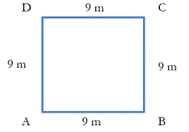
\includegraphics[width=0.4\columnwidth]{bab2/Gambar/Picture48.png}
				\end{center}
				\vspace{-0.2cm}
				%\rule{\columnwidth}{0.1pt}
				\captionsetup{justification=centering}
				\caption{Pola Jarak Tanam Bujur Sangkar atau Segiempat}\label{img:Pola-Jarak-Tanam-Bujur}
			\end{figure}
			%%%%%%%%%%%%%%%%%%%%%%%%%% GAMBAR %%%%%%%%%%%%%%%%%%%%%%%%%%%%%%
			Persamaan:
			\[ Jumlah\ Populasi=\ \frac{Luas\ Area\ (Ha)}{Jarak\ Tanam} \]
			
			Perhitungan:\\
			Luas area	: 1 ha = 10000 m2\\
			Jarak Tanam	: 9m x 9m

			\[ Jumlah\ Populasi=\ \frac{10000}{9\ x\ 9}=123\ Tanaman \]
			
			\item Perhitungan Segitiga
			
			Dalam memahami perhitungan jumlah pohon kelapa sawit, maka seperti Gambar \ref{img:Pola-Jarak-Tanam-Segitiga} segitiga sama sisi yang mewakili jarak antar tanaman kelapa sawit.
			
			%%%%%%%%%%%%%%%%%%%%%%%%%% GAMBAR %%%%%%%%%%%%%%%%%%%%%%%%%%%%%%
			\begin{figure}[H]
				\vspace{-0.1cm}
				%\rule{\columnwidth}{0.1pt}
				\begin{center}
					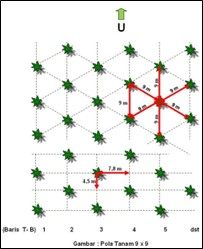
\includegraphics[width=0.4\columnwidth]{bab2/Gambar/Picture49.jpg}
				\end{center}
				\vspace{-0.2cm}
				%\rule{\columnwidth}{0.1pt}
				\captionsetup{justification=centering}
				\caption{Pola Jarak Tanam Segitiga\\(Sumber: GD Morganic, 2018)}\label{img:Pola-Jarak-Tanam-Segitiga}
			\end{figure}
			%%%%%%%%%%%%%%%%%%%%%%%%%% GAMBAR %%%%%%%%%%%%%%%%%%%%%%%%%%%%%%
			Dimana: 
			
			a: Jarak tanam\\
			b: Jarak antar baris yang akan dicari \\
			
			Persamaan:
			\[ Jumlah\ Populasi=\ \frac{Luas\ Area\ (Ha)}{a\ x\ b} \]
			
			Perhitungan:\\
			Luas area	: 1 ha = 10000 m2\\
			Jarak Tanam	: 9m x 9m x 9m
			
			\[ Jumlah\ Populasi=\ \frac{10000}{9\ x\ \sqrt{9^2-\ {4,5}^2}} \]
			\[ Jumlah\ Populasi=\ \frac{10000}{9\ x\ 7,79}=143\ Tanaman \]
			
			Dari kedua model tanam bujur sangkar dan segitiga dengan jarak tanam yang berbeda, maka populasi tanaman kelapa sawit segitiga lebih banyak dalam satuan luas hektar. Berdasarkan hubungan jarak taman, pola tanam, dan populasi hektar untuk tanaman kelapa sawit dapat diperkirakan seperti pada Tabel \ref{tbl:Hubungan-Jarak-Tanam-Populasi-Per-Hektar}.
			
			%%%%%%%%%%%%%%%%%%%%%%%TABEL SEDERHANA%%%%%%%%%%%%%%%%%%%%%%%%%
			\begin{singlespace}
				\begin{table}[H]
					\centering
					\caption{Hubungan Jarak Tanam dan Populasi per Hektar Kelapa Sawit}
					\label{tbl:Hubungan-Jarak-Tanam-Populasi-Per-Hektar}
					\begin{tabular}{|p{4cm}|p{3cm}|p{3cm}|}
						\hline
						\rowcolor[HTML]{C0C0C0} 
						Jarak Tanam (meter) & Bujur sangkar & Segitiga \\ \hline
						6                   & 278           & 320      \\ \hline
						7                   & 204           & 236      \\ \hline
						8                   & 156           & 180      \\ \hline
						9                   & 123           & 143      \\ \hline
					\end{tabular}
				\end{table}
			\end{singlespace}
			%%%%%%%%%%%%%%%%%%%%%%%TABEL SEDERHANA%%%%%%%%%%%%%%%%%%%%%%%%%
			
			Pada Tabel \ref{tbl:Hubungan-Jarak-Tanam-Populasi-Per-Hektar} dapat diketahui bahwa jarak tanam dengan model segitiga terbukti populasinya lebih banyak, hal ini disebabkan karena jarak tanam segitiga dapat memaksimalkan ruan yang ada dalam menangkap sinar matahari, nutrisi, tanah, dan air dengan jalan mengurangi adanya ruang kosong, serta tajuk tiak saling menutupi. 
			
		\end{enumerate}
		
	\end{enumerate}
\end{enumerate}

\section{\textit{State of The Art} (Penelitian Terdahulu)}
\hspace{1,2cm}Beberapa penelitian yang telah dilakukan berkenaan dengan kkelapa sawit dirangkum dalam Tabel 2.6. berikut ini: 

%%%%%%%%%%%%%%%%%%%%%%%TABEL SEDERHANA%%%%%%%%%%%%%%%%%%%%%%%%%
\begin{singlespace}
	\begin{table}[H]
		\centering
		\caption{\textit{State of the Art} (Penelitian Terdahulu)h}
		\label{tbl:Start-of-The-Art}
		\begin{tabular}{|p{2cm}|p{2cm}|p{2cm}|p{2cm}|p{2cm}|}	
			\hline
			Tahun & Penulis & Judul & Metode & Hasil \\ \hline
			2015  & Wong-in, T. Kaewkongka, T., Nagul C.,   Rajalida L.                    & Automatic Oil Palm Detection and Identification from Multi-Scale Clustering and Normalized Cross Correlation                                         & Noise filtering dengan spatial domain dan Gaussian smoothing. Untuk Eliminasi Non-Oil Palm dengan Gaussian Blurre image (Black-White), dan Identifikasi Oil Palm dengan K-Means & Wilayah yang diambil dari 21 gambar udara oil palm plantation berbeda region di Thailand dengan Camera Digital pada remote airplane. Penelitian ini dapat mendeteksi dan mengidentifikasi oil palm dengan akurasi di atas 90\%.                                                                                   \\ \hline
			\end{tabular}
	\end{table}
\end{singlespace}
%%%%%%%%%%%%%%%%%%%%%%%TABEL SEDERHANA%%%%%%%%%%%%%%%%%%%%%%%%%

%%%%%%%%%%%%%%%%%%%%%%%TABEL SEDERHANA%%%%%%%%%%%%%%%%%%%%%%%%%
\begin{singlespace}
	\begin{table}[H]
		\centering
		%\caption{\textit{State of the Art} (Penelitian Terdahulu)h}
		%\label{tbl:Start-of-The-Art}
		\begin{tabular}{|p{2cm}|p{2cm}|p{2cm}|p{2cm}|p{2cm}|}	
			\hline
			Tahun & Penulis & Judul & Metode & Hasil \\ \hline
			2016  & H. Santoso, H. Tani, X. Wang                                           & A simple method for detection and counting of oil palm trees using high-resolution multispectral satellite imagery                                   & BW, Pansharpening, Hue Saturation, ArcGIS                                                                                                                                       & Dataset yang digunakan dari data gambar Satelit Quickbird dengan Pansharpening, Sobel Edge Detector, dan ArcGIS 10.2.2. Hasil penelitian ini mencapai akurasi 98\%.                                                                                                                                               \\ \hline
			2018  & H. M. Rizeei, H. Z. M. Shafri, M. A. Mohamoud, B. Pradhan, B. Kalantar & Oil Palm Counting and Age Estimation from WorldView-3 Imagery and LiDAR Data Using an Integrated OBIA Height Model and Regression Analysis.          & SVM dan Regressi Analysis                                                                                                                                                       & Dataset menggunakan gambar satelit WV-3 dan Light Detection and Range (LiDAR). Hasil penelitian ini mendekati 99\%.                                                                                                                                                                                               \\ \hline
			2019  & N. A. Mubin, E. Nadarajoo, H. Z. M. Shafri, and A. Hamedianfar         & Young and Mature Oil Palm Tree Detection and Counting Using Convolutional Neural Network Deep Learning                                               & CNN, GIS                                                                                                                                                                        & Muda: 95,11\% Matang: 92,96\%                                                                                                                                                                                                                                                                                     \\ \hline
		\end{tabular}
	\end{table}
\end{singlespace}
%%%%%%%%%%%%%%%%%%%%%%%TABEL SEDERHANA%%%%%%%%%%%%%%%%%%%%%%%%%

%%%%%%%%%%%%%%%%%%%%%%%TABEL SEDERHANA%%%%%%%%%%%%%%%%%%%%%%%%%
\begin{singlespace}
	\begin{table}[H]
		\centering
		%\caption{\textit{State of the Art} (Penelitian Terdahulu)h}
		%\label{tbl:Start-of-The-Art}
		\begin{tabular}{|p{2cm}|p{2cm}|p{2cm}|p{2cm}|p{2cm}|}	
			\hline
			Tahun & Penulis & Judul & Metode & Hasil \\ \hline
			2020  & J. Zheng, H. Fu, W. Lo, W. Wu, Y. Zhao, R.   Dong, L. Yu..             & Cross-Regional Oil Palm Tree Counting and Detection via Multi-Level Attention Domain Adaptation Network                                              & Multi-Level Attention Domain Adaption Network (MADAN)                                                                                                                           & Dengan cross lokasi. Eksperimen dengan 3 large scale gambar satelit dari kelapa sawit di Peninsular Malaysia dengan berbeda lokasi. Dataset yang digunakan dengan annonated (label) yang sudah diberikan pada proses labeling. MADAN mendapatkan hasil rata-rata F1-Score 84.81\% tanpa target domain annotation. \\ \hline
		\end{tabular}
	\end{table}
\end{singlespace}
%%%%%%%%%%%%%%%%%%%%%%%TABEL SEDERHANA%%%%%%%%%%%%%%%%%%%%%%%%%

%%%%%%%%%%%%%%%%%%%%%%%TABEL SEDERHANA%%%%%%%%%%%%%%%%%%%%%%%%%
\begin{singlespace}
	\begin{table}[H]
		\centering
		%\caption{\textit{State of the Art} (Penelitian Terdahulu)h}
		%\label{tbl:Start-of-The-Art}
		\begin{tabular}{|p{2cm}|p{2cm}|p{2cm}|p{2cm}|p{2cm}|}	
			\hline
			Tahun & Penulis & Judul & Metode & Hasil \\ \hline
			2021  & X. Liu, K. H. Ghazali, F. Han, I. I. Mohamed                           & Automatic Detection of Oil Palm Tree from UAV Images Based on the Deep Learning Method                                                               & Faster RCNN                                                                                                                                                                     & Dataset yang digunakan dari UAV dengan gambar mencakup 22 hektar oil palm tree plantation. Hasil menunjukkan bahwa OA (overall accuracy sebesar 96\%.                                                                                                                                                             \\ \hline
			2021  & Y. Nurmasari, A. W. Wijayanto                                          & Oil Palm Plantation Detection in Indoensia Using Sentinel-2 and Landsat-8 Optical Setllite Imagery (Case Study: Rokan   Hulu Regency, Riau Province) & Supervised ML (Decision tree, Random Forest, Support Vector Machine, dan Naïve Bayes).                                                                                          & Dataset diambil dari Google Earth Engine   (GEE) untuk Google Earth, Sentinel-2 dan Landsat-8. Sentinel-2 tercatat 92\% tertinggi dengan Random Forest, dan Landsat-8 tercatat 66\%.                                                                                                                              \\ \hline
		\end{tabular}
	\end{table}
\end{singlespace}
%%%%%%%%%%%%%%%%%%%%%%%TABEL SEDERHANA%%%%%%%%%%%%%%%%%%%%%%%%%

%%%%%%%%%%%%%%%%%%%%%%%TABEL SEDERHANA%%%%%%%%%%%%%%%%%%%%%%%%%
\begin{singlespace}
	\begin{table}[H]
		\centering
		%\caption{\textit{State of the Art} (Penelitian Terdahulu)h}
		%\label{tbl:Start-of-The-Art}
		\begin{tabular}{|p{2cm}|p{2cm}|p{2cm}|p{2cm}|p{2cm}|}	
			\hline
			Tahun & Penulis & Judul & Metode & Hasil \\ \hline
			2022  & H. Wibowo, I. S. Sitanggang, M. Mushthofa, H. A. Adrianto. 2022.       & Large-Scale Oil Palm Trees Detection from High-Resloution Remote Sensing Images Using Deep Learning                                                  & YOLOv3, YOLOv4, YOLOv5                                                                                                                                                          & Akurasi yang dicapai pada penelitian ini YOLOv4: 97.28\%, YOLOv4: 97.74\%, dan YOLOv5: 94.94\%                                                                                                                                                                                                                    \\ \hline
			2023  & S. Munir, K. B. Seminar, Sudradjat, H. Sukoco, A. Buono                & The Use of Random Forest Regression for Estimating Leaf Nitrogen Content of Oil Palm Based on Sentinel 1-A Imagery                                   & Random Forest Regression                                                                                                                                                        & Penilaian kinerja model memperoleh rata-rata MAPE, koreksi, dan MSE 9,68\%, 90.32\% dan 11.03\%. Peta spasial dari distribusi nilai nitrogen di daerah dapat diproduksi dan divisualisasikan di web sehingga dapat diakses dengan mudah dan cepat untuk pengolahan.                                               \\ \hline
		\end{tabular}
	\end{table}
\end{singlespace}
%%%%%%%%%%%%%%%%%%%%%%%TABEL SEDERHANA%%%%%%%%%%%%%%%%%%%%%%%%%